\documentclass[8pt,aspectratio=169]{beamer}
\usetheme{Boadilla}

\usepackage{hyperref}
\usepackage{graphicx}
\usepackage{subfig}
\usepackage{amsmath,amssymb}

\graphicspath{ {images/} }

\usepackage{tikz}

%Some useful commands for QM
\newcommand{\bra}[1]{\left< #1 \right|}
\newcommand{\ket}[1]{\left| #1 \right>}
\newcommand{\expVal}[1]{\left< #1 \right>}
\newcommand{\braket}[2]{\left<#1|#2\right>}

%Stolen from http://tex.stackexchange.com/questions/178800/creating-sections-each-with-title-pages-in-beamers-slides
\AtBeginSection[]{
  \begin{frame}
  \vfill
  \centering
  \begin{beamercolorbox}[sep=8pt,center,shadow=true,rounded=true]{title}
    \usebeamerfont{title}\insertsectionhead\par%
  \end{beamercolorbox}
  \vfill
  \end{frame}
}

\title{Holographic Complexity}
\author{Josiah Couch}
\institute{University of Texas at Austin}
%\institute{At Oklahoma State University}
\date{24 April 2018}



\begin{document}

\begin{frame}
\titlepage\end{frame}

\begin{frame}
\frametitle{Outline}
\tableofcontents[]
\end{frame}

\section{Introduction}

\subsection{Black Holes and Holography}

%\begin{frame}
%\frametitle{Overview of BH Thermodyamics}

%\begin{itemize}

%\item Second law of black holes

%\item First law of black hole thermodynamics

%\item Hawking radiation

%\item Black hole thermodynamics

%\item Entropy bounds

%\item Holographic principle?

%\end{itemize}

%\end{frame}

\begin{frame}
\frametitle{The AdS/CFT Correspondence}

In 1999, Juan Maldacena argued based on string theory that $\mathcal{N}=4$ super Yang-Mills (SYM) in $3+1$ dimensions with gauge group SU($N$) is dual to type IIB string theory on $AdS_5\times S^5$. This became the first example of so-called AdS/CFT duality between a gravity theory in an asymptotically anti de-Sitter (AdS) space time (times a compact manifold) and a conformal field theory (CFT) living 'on the conformal boundary' of that spacetime. 

\begin{itemize}

\item These theories are dual in that the partition functions are 'the same'.

\item In a certain limit (usually taken), the rank $N$ of the gauge group becomes large, and the string theory approximately reduces to classical Einstein gravity.

\item At low energies we can get rid of compact manifold by a Kaluza-Klein reduction.

\item When the field theory is strongly coupled, gravity theory is weakly coupled.

\item So in the end we have a duality between a strongly coupled field theory in $d$ dimensions and classical gravity (plus KK modes) in asymptotic $AdS_{d+1}$.

\item UV of the field theory becomes IR of the gravity theory.

\item A particular classical geometry is actually dual to a particular (possibly time dependent) state on the boundary.

\end{itemize}

\end{frame}

%\begin{frame}
%\frametitle{The AdS/CFT Correspondence}

%The AdS/CFT correspondence was first proposed in 1999 by Juan Maldacena. It is a holographic duality between a conformal field theory (CFT) in d dimensions, refered to as the boundary theory, and quantum gravity in a d+1 dimensional asymptotically anti de Sitter (AdS) spacetime, which is dubbed the bulk. 

%\begin{itemize}

%\item The original version, proposed by Maldacena in 1999, is a duality between $\mathcal{N}=4$ super Yang-Mills (SYM) in 3+1 dimensions and type IIB string theory on $AdS_5\times S^5$

%\item This was derived by considering a stack of D3-branes in the coincident limit: The 'boundary' theory is simply the worldvolume theory, and the bulk theory comes from considering the near horizon geometry of the stack.

%\item In the limit where the rank of the boundary gauge group becomes large, the bulk is well described by classical (super) gravity.

%\item This duality relates strong coupling on the boundary to weak couplling in the bulk, and the UV on the boundary to the IR in the bulk.

%\item $1/N$ corrections in the boundary theory correspond to quantum corrections in the bulk.

%\item This original duallity has been extended in many ways

%\begin{itemize}

%	\item One can consider different versions of the stringy setup, i.e. D2-branes in type IIA, or M-branes in 11d M theory
	
%	\item Recently there has been interest in getting $AdS_2$ diliton gravity from the $0+1$ dimensional Sachdev-Ye-Kitaev (SYK) model. 
	
%	\item It is generally believed that any asymptotically AdS spacetime which is a solution for some gravity theory will have a CFT dual

%\end{itemize}

%\end{itemize}

%\end{frame}

\begin{frame}
\frametitle{Applications of the AdS/CFT Correspondence}

One important application of AdS/CFT has been to study strongly coupled  field theories.

\begin{itemize}

\item Boundary theory is an SU($N$) gauge theory, so there have been attempts to use AdS/CFT to study QCD at strong coupling.

\item There is a hope to be able to understand strongly coupled condensed matter systems. 

\item In particular, it is easy to study the entanglement structure of the boundary state in AdS/CFT

\end{itemize}

On the other hand, there is an effort to use AdS/CFT to say something about quantum gravity.

\begin{itemize}

\item AdS/CFT would seem to imply black holes are goverened by unitary dynamics, contrary to arguments by e.g. Hawking.

\item There has been work deriving the einstein equations as a consequence of the first law of entanglement entropy on the boundary. 

\item Perhaps geometry emerges from the entanglement structure of quantum UV degrees of freedom?

\end{itemize}

\end{frame}

\begin{frame}
\frametitle{Thermodynamics in AdS/CFT}

Under the AdS/CFT dictionary, a black hole in the bulk is dual to a thermal state on the boundary, with the temperature, entropy, etc. of the boundary state identical to those of the black hole.

\begin{itemize}

\item Consider an asymptotically AdS black hole geometry: $ds^2 = - f(r) dt^2 + \frac{dr^2}{f(r)} + r^2 d\Omega^2$

\item Wick rotating to euclidean time $t_E$, we see that in order to avoid a conical singularity at the horizon, we must identify $t_E \sim t_E + \beta$, with $\beta$ the inverse black hole temperature. 

\item Because the bulk and boundary partition functions are the same, we have in a saddle point approximation $\ln(Z) \approx - S_\text{cl}$, where $S_\text{cl}$ is the Euclidean Einstein-Hilbert action evaluated on our particular solution.

\item Evaluating $U = - \frac{\partial \ln Z}{\partial \beta}$, we find that $U := \expVal{H} = M$, where $H$ is the boundary Hamiltonian, and and $M$ is the mass of the black hole.

\item Similarly, one may find the entropy by $S = -\frac{\partial (T \ln Z)}{\partial T}$ to discover that the entropy of the boundary state is simply the entropy of the black hole.

\item We likewise have that the charge of the black hole is dual to the boundary chemical potential.

\end{itemize}

\end{frame}

\begin{frame}
\frametitle{Entanglement and Bulk Reconstruction}

I mentioned before that AdS/CFT can also give the entanglement structure of the boundary state. This is given by the so called Ryu-Takayanagi prescription: 

\begin{minipage}[t]{0.55\linewidth}

\end{minipage}\hfill
%
\begin{minipage}[t]{0.44\linewidth}

\begin{figure}
    \begin{center}
    
        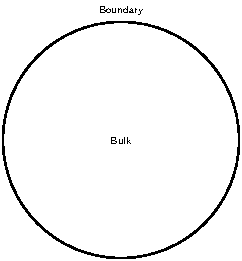
\includegraphics[scale=1]{RT0}    
    
    \end{center}
    \caption{The Ryu-Takayanagi Prescription}
    \label{fig:WDW}
\end{figure}

\end{minipage}

\end{frame}

\begin{frame}
\frametitle{Entanglement and Bulk Reconstruction}

I mentioned before that AdS/CFT can also give the entanglement structure of the boundary state. This is given by the so called Ryu-Takayanagi prescription: 

\begin{minipage}[t]{0.55\linewidth}

\begin{itemize}

\item Consider a spatial slice of our AdS spacetime

\end{itemize}

\end{minipage}\hfill
%
\begin{minipage}[t]{0.44\linewidth}

\begin{figure}
    \begin{center}
    
        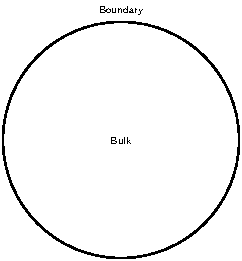
\includegraphics[scale=1]{RT0}    
    
    \end{center}
    \caption{The Ryu-Takayanagi Prescription}
    \label{fig:WDW}
\end{figure}

\end{minipage}

\end{frame}

\begin{frame}
\frametitle{Entanglement and Bulk Reconstruction}

I mentioned before that AdS/CFT can also give the entanglement structure of the boundary state. This is given by the so called Ryu-Takayanagi prescription: 

\begin{minipage}[t]{0.55\linewidth}

\begin{itemize}

\item Consider a spatial slice of our AdS spacetime

\item On this spatial slice, specify a boundary region $A$, whose entanglement entropy we want to compute. 

\end{itemize}

\end{minipage}\hfill
%
\begin{minipage}[t]{0.44\linewidth}

\begin{figure}
    \begin{center}
    
        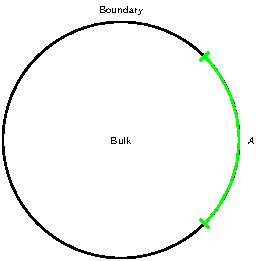
\includegraphics[scale=1]{RT1}    
    
    \end{center}
    \caption{The Ryu-Takayanagi Prescription}
    \label{fig:WDW}
\end{figure}

\end{minipage}

\end{frame}

\begin{frame}
\frametitle{Entanglement and Bulk Reconstruction}

I mentioned before that AdS/CFT can also give the entanglement structure of the boundary state. This is given by the so called Ryu-Takayanagi prescription: 

\begin{minipage}[t]{0.55\linewidth}

\begin{itemize}

\item Consider a spatial slice of our AdS spacetime

\item On this spatial slice, specify a boundary region $A$, whose entanglement entropy we want to compute. 

\item Consider the surface of minimal area whose boundary intersects that of our region A. We will call this the RT surface for $A$

\end{itemize}

\end{minipage}\hfill
%
\begin{minipage}[t]{0.44\linewidth}

\begin{figure}
    \begin{center}
    
        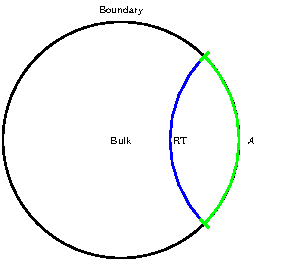
\includegraphics[scale=1]{RT}    
    
    \end{center}
    \caption{The Ryu-Takayanagi Prescription}
    \label{fig:WDW}
\end{figure}

\end{minipage}

\end{frame}

\begin{frame}
\frametitle{Entanglement and Bulk Reconstruction}

I mentioned before that AdS/CFT can also give the entanglement structure of the boundary state. This is given by the so called Ryu-Takayanagi prescription: 

\begin{minipage}[t]{0.55\linewidth}

\begin{itemize}

\item Consider a spatial slice of our AdS spacetime

\item On this spatial slice, specify a boundary region $A$, whose entanglement entropy we want to compute. 

\item Consider the surface of minimal area whose boundary intersects that of our region A. We will call this the RT surface for $A$

\item The entanglement entropy of $A$ is then the area of the RT surface over $4\pi G$.

\end{itemize}

\end{minipage}\hfill
%
\begin{minipage}[t]{0.44\linewidth}

\begin{figure}
    \begin{center}
    
        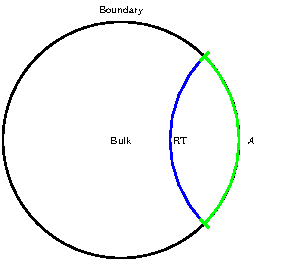
\includegraphics[scale=1]{RT}    
    
    \end{center}
    \caption{The Ryu-Takayanagi Prescription}
    \label{fig:WDW}
\end{figure}

\end{minipage}

\end{frame}

\begin{frame}
\frametitle{Entanglement and Bulk Reconstruction}

I mentioned before that AdS/CFT can also give the entanglement structure of the boundary state. This is given by the so called Ryu-Takayanagi prescription: 

\begin{minipage}[t]{0.55\linewidth}

\begin{itemize}

\item Consider a spatial slice of our AdS spacetime

\item On this spatial slice, specify a boundary region $A$, whose entanglement entropy we want to compute. 

\item Consider the surface of minimal area whose boundary intersects that of our region A. We will call this the RT surface for $A$

\item The entanglement entropy of $A$ is then the area of the RT surface over $4\pi G$.

\item The causal development of the spatial region bounded by the RT surface is called the \textit{entanglement wedge}

\end{itemize}

\end{minipage}\hfill
%
\begin{minipage}[t]{0.44\linewidth}

\begin{figure}
    \begin{center}
    
        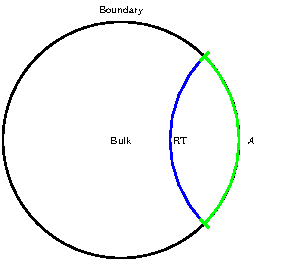
\includegraphics[scale=1]{RT}    
    
    \end{center}
    \caption{The Ryu-Takayanagi Prescription}
    \label{fig:WDW}
\end{figure}

\end{minipage}

\end{frame}

\begin{frame}
\frametitle{Entanglement and Bulk Reconstruction}

I mentioned before that AdS/CFT can also give the entanglement structure of the boundary state. This is given by the so called Ryu-Takayanagi prescription: 

\begin{minipage}[t]{0.55\linewidth}

\begin{itemize}

\item Consider a spatial slice of our AdS spacetime

\item On this spatial slice, specify a boundary region $A$, whose entanglement entropy we want to compute. 

\item Consider the surface of minimal area whose boundary intersects that of our region A. We will call this the RT surface for $A$

\item The entanglement entropy of $A$ is then the area of the RT surface over $4\pi G$.

\item The causal development of the spatial region bounded by the RT surface is called the \textit{entanglement wedge}

\item The mixed state on $A$ is dual the the entanglement wedge of $A$.

\end{itemize}

\end{minipage}\hfill
%
\begin{minipage}[t]{0.44\linewidth}

\begin{figure}
    \begin{center}
    
        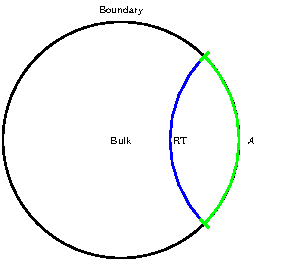
\includegraphics[scale=1]{RT}    
    
    \end{center}
    \caption{The Ryu-Takayanagi Prescription}
    \label{fig:WDW}
\end{figure}

\end{minipage}

\end{frame}

\begin{frame}
\frametitle{Entanglement and Bulk Reconstruction}

I mentioned before that AdS/CFT can also give the entanglement structure of the boundary state. This is given by the so called Ryu-Takayanagi prescription: 

\begin{minipage}[t]{0.55\linewidth}

\begin{itemize}

\item Consider a spatial slice of our AdS spacetime

\item On this spatial slice, specify a boundary region $A$, whose entanglement entropy we want to compute. 

\item Consider the surface of minimal area whose boundary intersects that of our region A. We will call this the RT surface for $A$

\item The entanglement entropy of $A$ is then the area of the RT surface over $4\pi G$.

\item The causal development of the spatial region bounded by the RT surface is called the \textit{entanglement wedge}

\item The mixed state on $A$ is dual the the entanglement wedge of $A$.

\end{itemize}

\end{minipage}\hfill
%
\begin{minipage}[t]{0.44\linewidth}

\begin{figure}
    \begin{center}
    
        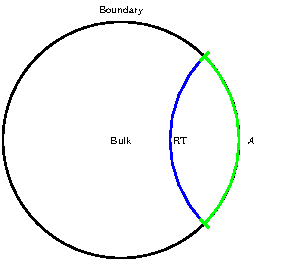
\includegraphics[scale=1]{RT}    
    
    \end{center}
    \caption{The Ryu-Takayanagi Prescription}
    \label{fig:WDW}
\end{figure}

\end{minipage}

By considering all possible subregions and their respective entanglement entropies, we may hope to reconstruct the dual bulk geometry from field theory data.

\end{frame}

\begin{frame}
\frametitle{Behind the BH Horizon}

We state before that a black hole geometry is dual to a thermal state. Strictly speaking, it is geometry outside the horizon which is dual to a thermal state.

\begin{minipage}[t]{0.55\linewidth}

\begin{itemize}

\item The (geodesically) complete geometry is a two sided black hole geometry

\item This geometry has two boundaries, with a CFT  on each boundary. The Hilbert space is given by $\mathcal{H} = \mathcal{H}_L \otimes \mathcal{H}_R$

\item The state dual to this configuration is a purification of the thermal state known as the thermofield double state: 

$$\psi = \displaystyle\sum_n e^{- \beta E_n /2} \ket{E_n}_L \otimes \ket{E_n}_R$$

\item Outside of horizon geometry corresponds in some sense to the entanglement structure of the thermal state.

\item What about the the geometry behind the horizon?

\end{itemize}

\end{minipage}\hfill
%
\begin{minipage}[t]{0.44\linewidth}

\begin{figure}
    \begin{center}
    
        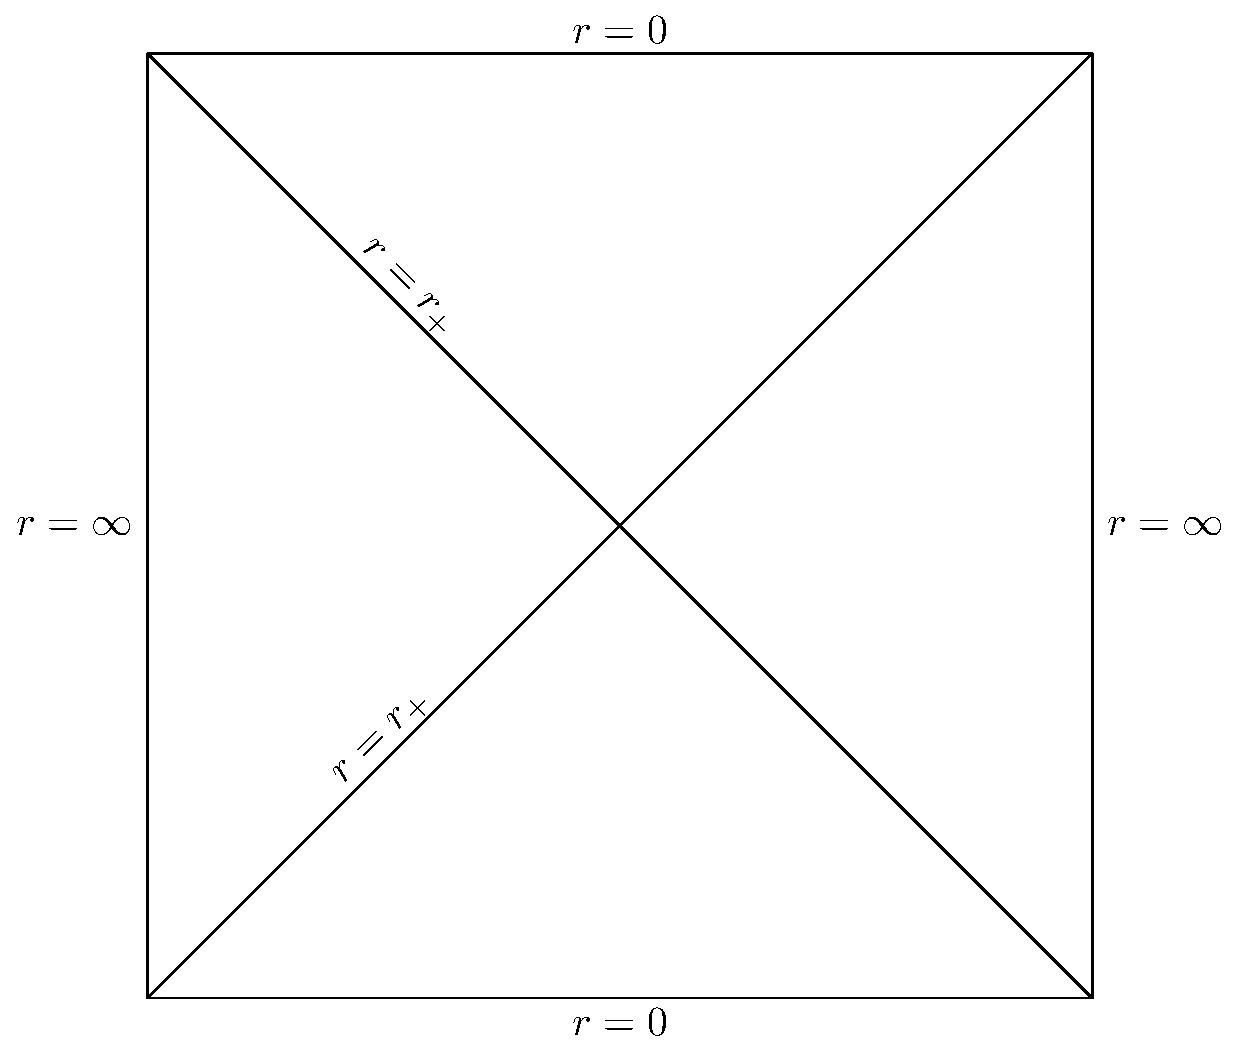
\includegraphics[scale=0.3]{2SidedBH}    
    
    \end{center}
    \caption{Two sided black hole}
    \label{fig:WDW}
\end{figure}

\end{minipage}

\end{frame}

\subsection{Holographic Complexity}

\begin{frame}
\frametitle{Holographic Complexity}

There are some puzzling aspects to the behind the horizon geometry

\begin{minipage}[t]{0.55\linewidth}

\begin{itemize}

\item No region defined entirely on the left or right side is sensitive to this part of the geometry

\item The volume behind the horizon on a spatial slice continues growing long past the thermal time.

\end{itemize}

To resolve these issues, Leonard Susskind proposed that the geometry behind the horizon is dual to the \textit{quantum circuit complexity} of the dual state.

\begin{itemize}

\item Specifically, Susskind proposed that the complexity of boundary state is dual to the volume of a maximal spatial slice of the bulk. (Complexity = volume)

\item Like the volume, the complexity of the state obtained from the TFD state by unitary time evolution is expected to incrase long past the thermalization time

\item In fact it should grow for a time exponential in the number of degrees of freedom

\item Most of the increase in such a slice with time occurs behind the horizon.

\end{itemize}

\end{minipage}\hfill
%
\begin{minipage}[t]{0.44\linewidth}

\begin{figure}
    \begin{center}
    
        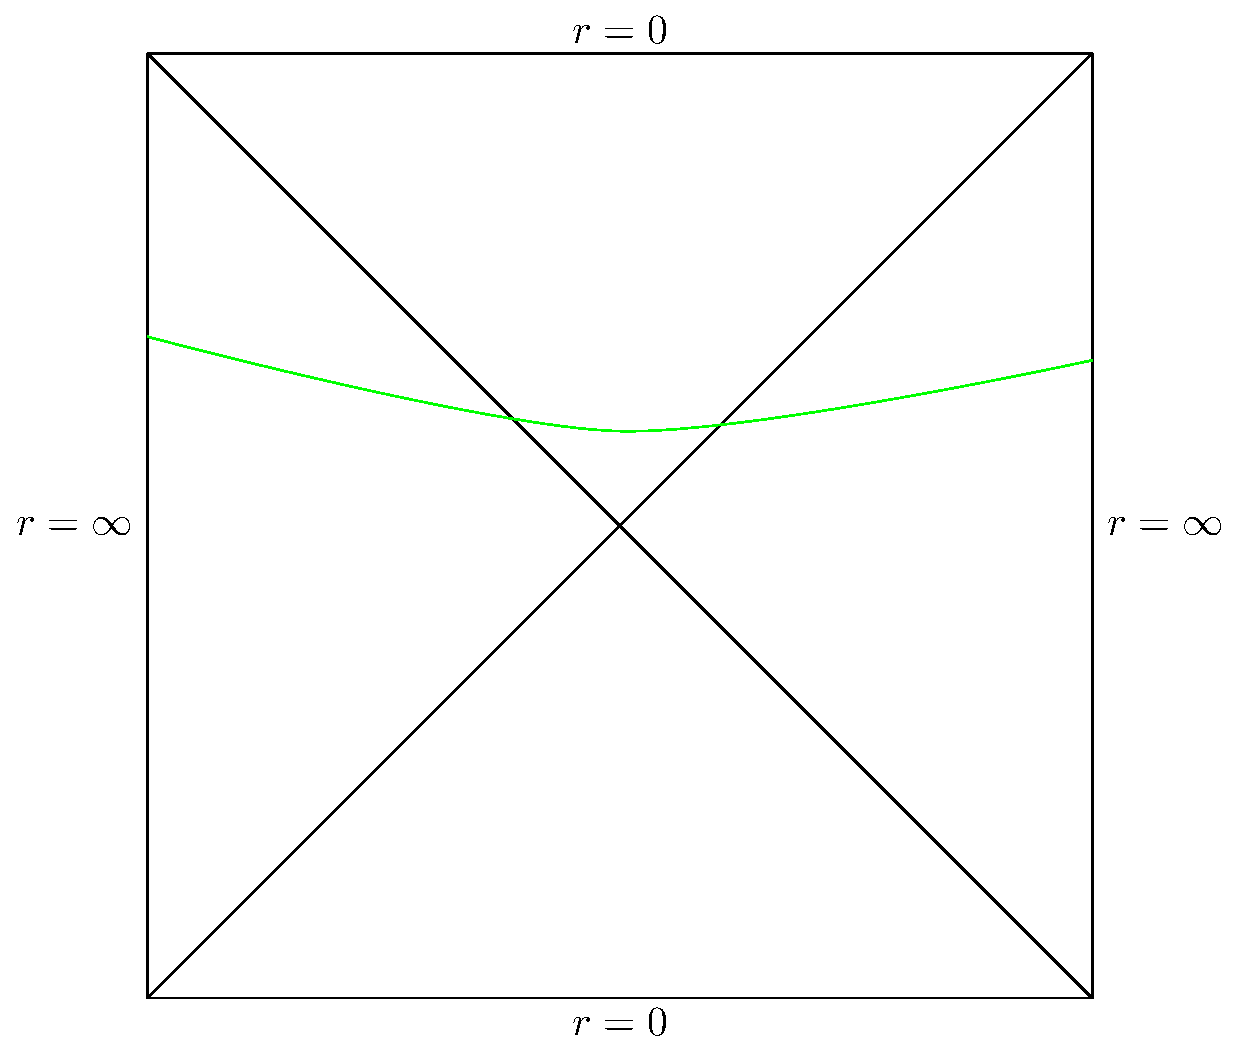
\includegraphics[scale=0.3]{CV}     
    
    \end{center}
    \caption{Maximal spatial slice}
    \label{fig:WDW}
\end{figure}

\end{minipage}

\end{frame}

\begin{frame}
\frametitle{Quantum Circuit Complexity}

What is circuit complexity?

\begin{itemize}

\item Consider a Hilbert space $\mathcal{H}$, e.g., the Hilbert space for $N$ quantum bits.

\item A universal gate set $\{g_i\}$ for $\mathcal{H}$ is a set of unitary operators on the Hilbert space such that any unitary $U$ acting on $\mathcal{H}$ can be approximated by some product $\displaystyle\prod_{i} g_{\alpha_i}$ to within a small tolerance $\epsilon$. 

\item Such a product of gates is referred to as a quantum circuit.

\item The quantum circuit complexity of a unitary $U$ is then the minimum number of gates needed to approximate $U$ to within the tolerance.

\item In the example of qubits, one typically considers gates that act on a single qubit or pairs of qubits at a time.

\item Given some reference state $\ket{\psi_R}$, one may define the complexity of a state $\ket{\psi}$ as the minimum of complexity $C(U)$ over all unitaries $U$ such that $\ket{\psi} = U\ket{\psi_R}$.

\end{itemize}

\end{frame}

\begin{frame}
\frametitle{The Switchback (Butterfly) effect}

\begin{itemize}

\item Given the time evolution operator $U(t)$ and some other operator $W$, we may construct a \textit{precursor operator} $U(t) W U(-t)$.

\item The expectation value of this operator is the overlap between the current state, and the state we would have obtained at the present had the operator $W$ been inserted a time $t$ in the past.

\item The complexity of this operator is lower bounded by the sum of the complexities of the individual operators: $\mathcal{C}(U(t)WU(-t))\leq 2 \mathcal{C}(U) + \mathcal{C}(W)$.

\item If $W$ is Haar random, this bound is saturated with overwhelming probabillity.

\item On the otherhand, clearly if $W$ is the identity the complexity is 0.

\item If $W$ is a local operator, then

\begin{itemize}

	\item for small $t$, the complexity is very small (nearly total cancelation).
	
	\item As $t$ increases, the local operator $W$ gets more and more scrambled over the whole Hilbert space.
	
	\item At large $t$ (much larger than the scrambling time), the complexity of the precursor operator grows at the same rate as ordinary time evolution. 

\end{itemize}

\item The insertion of an operator $W$ in the boundary theory in AdS/CFT is dual to a shockwave in the bulk originating at the boundary

\item Shockwave geometries may thus be used to test whether complexity = volume reproduces the switchback effect.

\item Complexity = volume has in fact been found to be consistent with the switchback effect in a wide variety of circumstances.

\end{itemize}

\end{frame}

\begin{frame}
\frametitle{Complexity = Action}

Complexity = volume has a few unpleasant features

\begin{itemize}

\item For example, in order to reproduce the correct boundary behavior, the volume must be multiplied by a non-universal length scale

\end{itemize}

One might seek an alternative proposal, which still captures something about the behind the horizon geometry, but which does not have these features. In fact, such an alternative has been proposed by Susskind et al., and it goes by 'complexity = action.'

\begin{itemize}

\item According to complexity = action, the complexity is dual to the action of a so-called 'Wheeler-DeWitt' (WDW) patch.

\item Because this is an action, it can be nondimensionalized with some multiple of $\hbar$. 

\item A universal choice for this coefficient is consistent with the expected large temperature behavior. 

\item The action of a WDW patch also behaves in the appropriate way in the presence of shockwaves, so it still reproduces the switchback effect.

\end{itemize}

\end{frame}

\begin{frame}
\frametitle{The WDW patch}

\begin{minipage}[t]{0.55\linewidth}

\begin{itemize}

\item The WDW patch is defined by a spatial slice of the boundary. 

\end{itemize}

\end{minipage}\hfill
%
\begin{minipage}[t]{0.44\linewidth}

\begin{figure}
    \begin{center}
    
        
\includegraphics[scale=0.4]{WDW0.pdf}    
    
    \end{center}
    \caption{Boundary times $t_L$ and $t_R$}
    \label{fig:WDW}
\end{figure}

\end{minipage}

\end{frame}


\begin{frame}
\frametitle{The WDW patch}

\begin{minipage}[t]{0.55\linewidth}

\begin{itemize}

\item The WDW patch is defined by a spatial slice of the boundary. 

\item For a two-sided black hole, this can be given by a left time $t_L$ and a right time $t_R$.

\end{itemize}

\end{minipage}\hfill
%
\begin{minipage}[t]{0.44\linewidth}

\begin{figure}
    \begin{center}
    
        
\includegraphics[scale=0.4]{WDW0.pdf}    
    
    \end{center}
    \caption{Boundary times $t_L$ and $t_R$}
    \label{fig:WDW}
\end{figure}

\end{minipage}

\end{frame}


\begin{frame}
\frametitle{The WDW patch}

\begin{minipage}[t]{0.55\linewidth}

\begin{itemize}

\item The WDW patch is defined by a spatial slice of the boundary. 

\item For a two-sided black hole, this can be given by a left time $t_L$ and a right time $t_R$.

\item The WDW patch is then defined as the union of all spatial slices which meet the left boundary at $t_L$ and the right boundary at $t_R$, along with the null boundary of this region.

\end{itemize}

\end{minipage}\hfill
%
\begin{minipage}[t]{0.44\linewidth}

\begin{figure}
    \begin{center}
    
        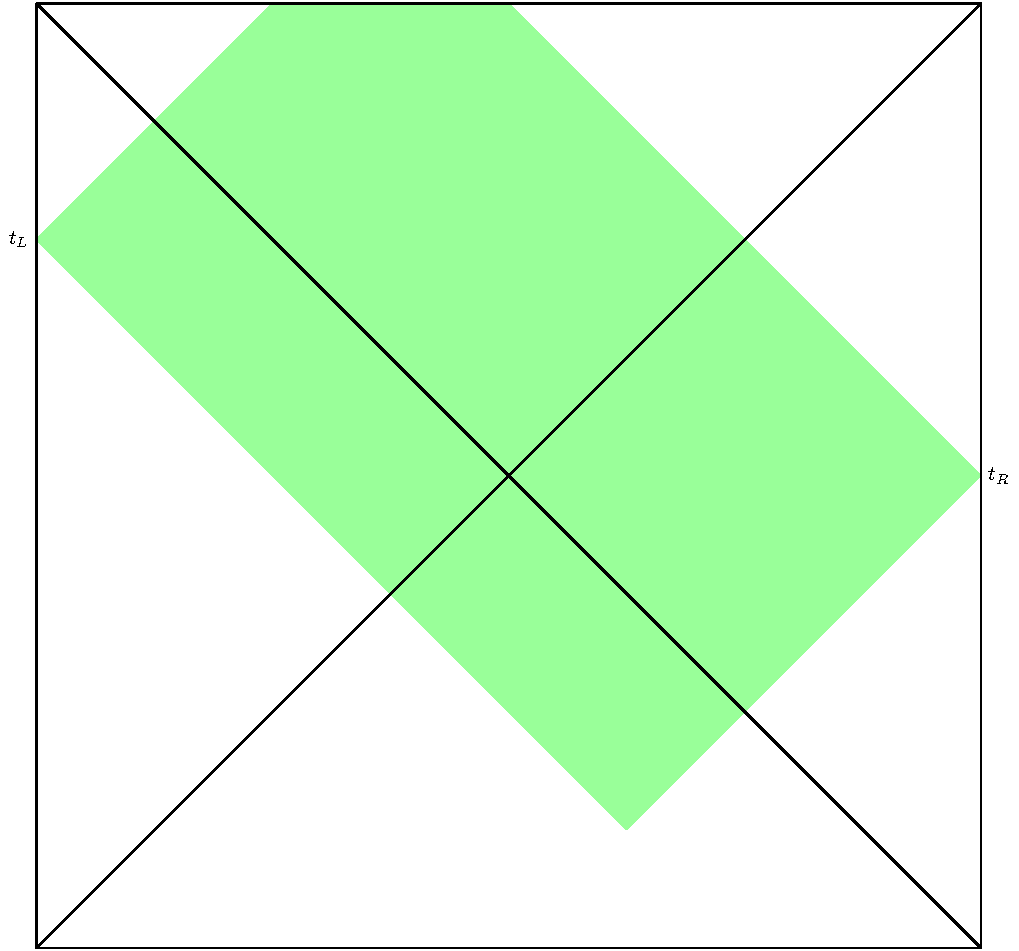
\includegraphics[scale=0.4]{WDW.pdf}    
    
    \end{center}
    \caption{The WDW patch defined by boundry times $t_L$ and $t_R$}
    \label{fig:WDW}
\end{figure}

\end{minipage}

\end{frame}


\begin{frame}
\frametitle{The WDW patch}

\begin{minipage}[t]{0.55\linewidth}

\begin{itemize}

\item The WDW patch is defined by a spatial slice of the boundary. 

\item For a two-sided black hole, this can be given by a left time $t_L$ and a right time $t_R$.

\item The WDW patch is then defined as the union of all spatial slices which meet the left boundary at $t_L$ and the right boundary at $t_R$, along with the null boundary of this region.

\item The action of this patch diverges at the boundary, so we will regularize by a cutoff

\end{itemize}

\end{minipage}\hfill
%
\begin{minipage}[t]{0.44\linewidth}

\begin{figure}
    \begin{center}
    
        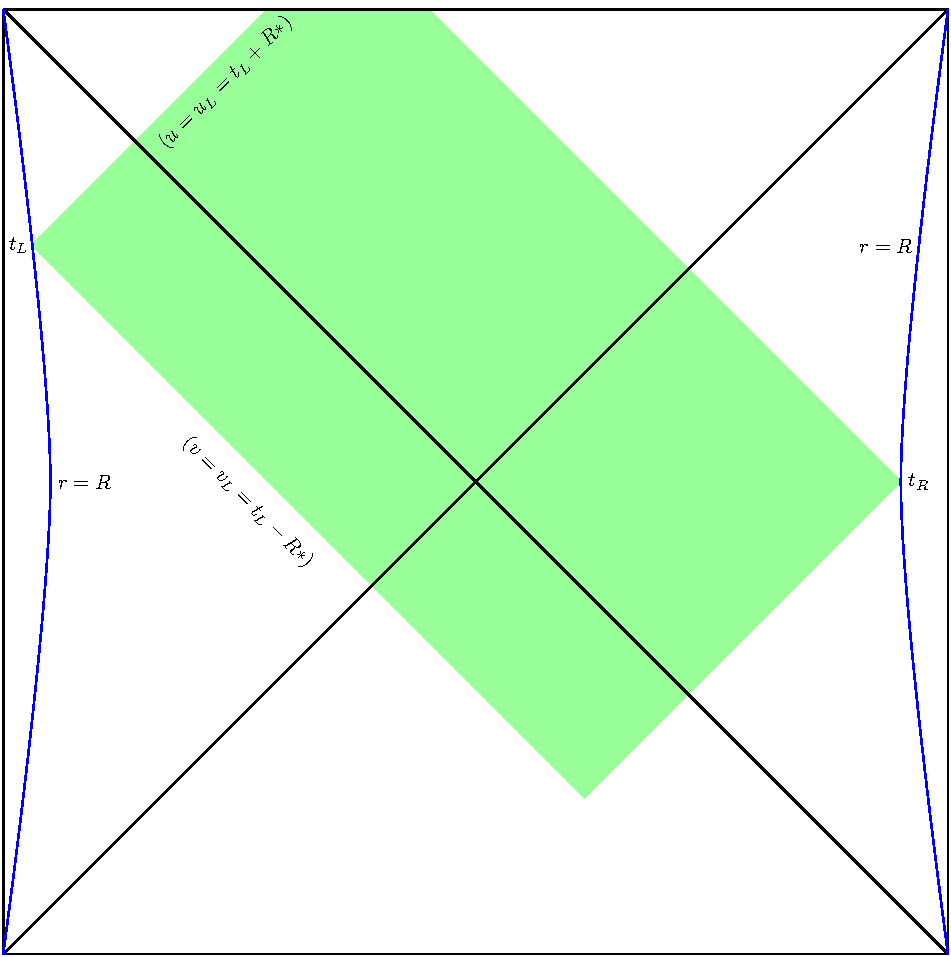
\includegraphics[scale=0.4]{WDW2.pdf}    
    
    \end{center}
    \caption{The WDW patch defined by boundry times $t_L$ and $t_R$ and a cutoff $R$}
    \label{fig:WDW2}
\end{figure}

\end{minipage}

\end{frame}


\begin{frame}
\frametitle{The WDW patch}

\begin{minipage}[t]{0.5\linewidth}

\begin{itemize}

\item The WDW patch is defined by a spatial slice of the boundary. 

\item For a two-sided black hole, this can be given by a left time $t_L$ and a right time $t_R$.

\item The WDW patch is then defined as the union of all spatial slices which meet the left boundary at $t_L$ and the right boundary at $t_R$, along with the null boundary of this region.

\item The action of this patch diverges at the boundary, so we will regularize by a cutoff

\item We will only be interested in the rate of change of the action, as $t_L$ increases.

\end{itemize}

\end{minipage}\hfill
%
\begin{minipage}[t]{0.48\linewidth}

\begin{figure}
    \begin{center}
    
        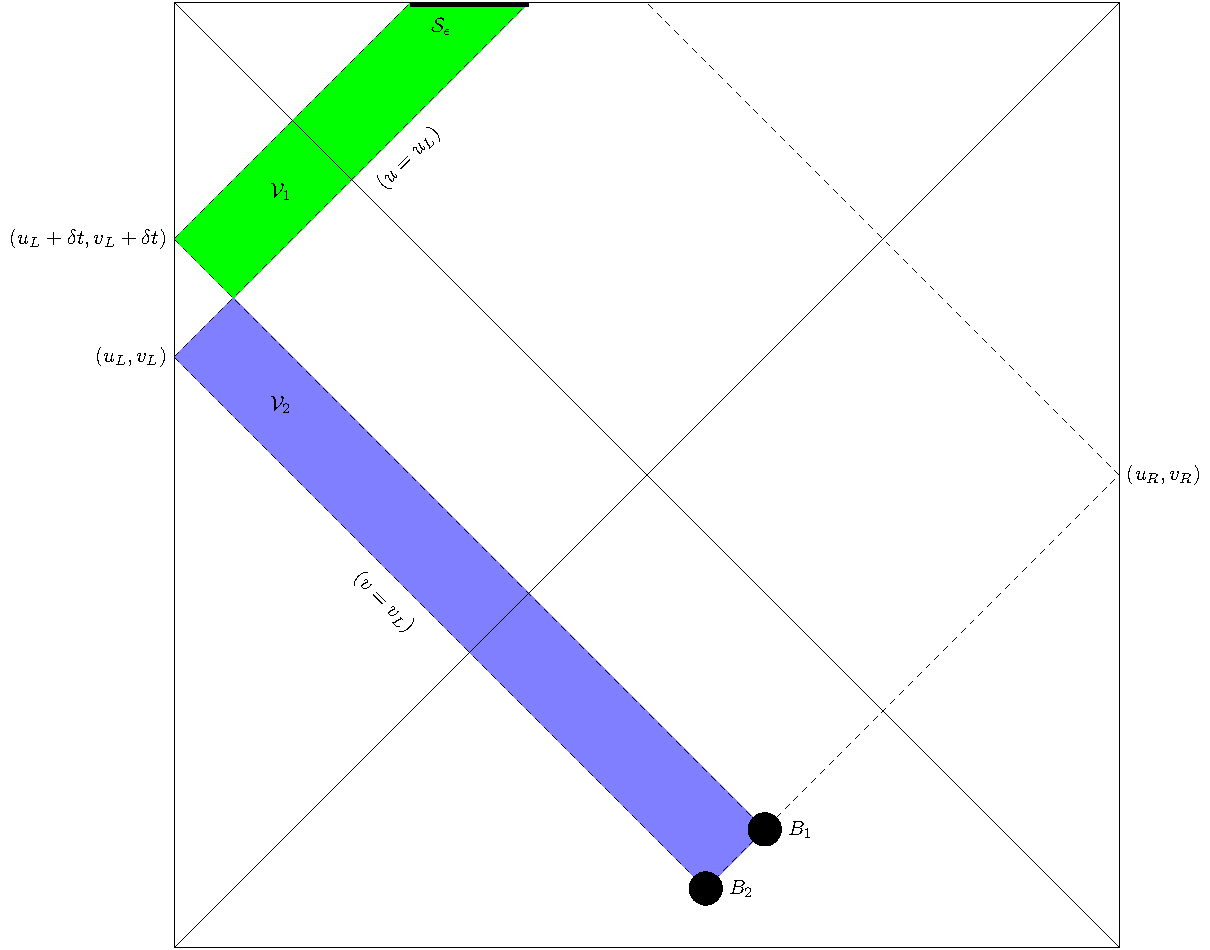
\includegraphics[scale=0.35]{2WDW.pdf}    
    
    \end{center}
    \caption{Two WDW patches separated by $\delta t$.  In thi figure, we have suppressed the cutoff}
    \label{fig:2WDW}
\end{figure}

\end{minipage}

\end{frame}


\begin{frame}
\frametitle{The WDW patch}

\begin{minipage}[t]{0.5\linewidth}

\begin{itemize}

\item The WDW patch is defined by a spatial slice of the boundary. 

\item For a two-sided black hole, this can be given by a left time $t_L$ and a right time $t_R$.

\item The WDW patch is then defined as the union of all spatial slices which meet the left boundary at $t_L$ and the right boundary at $t_R$, along with the null boundary of this region.

\item The action of this patch diverges at the boundary, so we will regularize by a cutoff

\item We will only be interested in the rate of change of the action, as $t_L$ increases.

\item This may be computed by subtracting the actions of two WDW patches, whose left time is separated by $\delta t$, and then taking the limit where $\delta t \rightarrow 0$.

\end{itemize}

\end{minipage}\hfill
%
\begin{minipage}[t]{0.48\linewidth}

\begin{figure}
    \begin{center}
    
        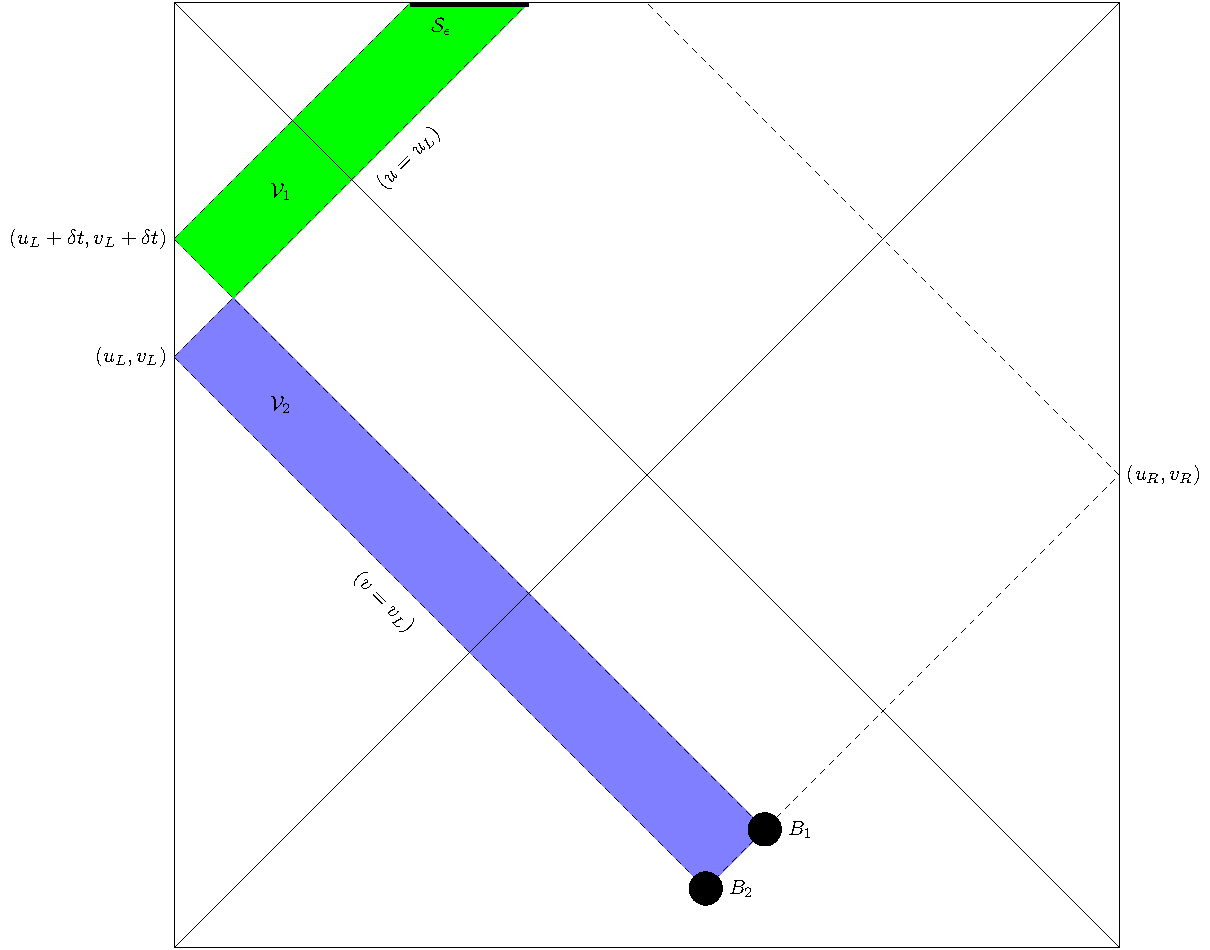
\includegraphics[scale=0.35]{2WDW.pdf}    
    
    \end{center}
    \caption{Two WDW patches separated by $\delta t$.  In thi figure, we have suppressed the cutoff}
    \label{fig:2WDW}
\end{figure}

\end{minipage}

\end{frame}


\begin{frame}
\frametitle{The WDW patch}

\begin{minipage}[t]{0.5\linewidth}

\begin{itemize}

\item The WDW patch is defined by a spatial slice of the boundary. 

\item For a two-sided black hole, this can be given by a left time $t_L$ and a right time $t_R$.

\item The WDW patch is then defined as the union of all spatial slices which meet the left boundary at $t_L$ and the right boundary at $t_R$, along with the null boundary of this region.

\item The action of this patch diverges at the boundary, so we will regularize by a cutoff

\item Often we will be interested in the rate of change of the action, as $t_L$ increases.

\item This may be computed by subtracting the actions of two WDW patches, whose left time is separated by $\delta t$, and then taking the limit where $\delta t \rightarrow 0$.

\item This difference of actions decomposes to the difference of two bulk pieces, a piece from the spacelike boundary of a near singularity cutoff, and two codimension two contributions from the past corners of the patches.

\end{itemize}

\end{minipage}\hfill
%
\begin{minipage}[t]{0.48\linewidth}

\begin{figure}
    \begin{center}
    
        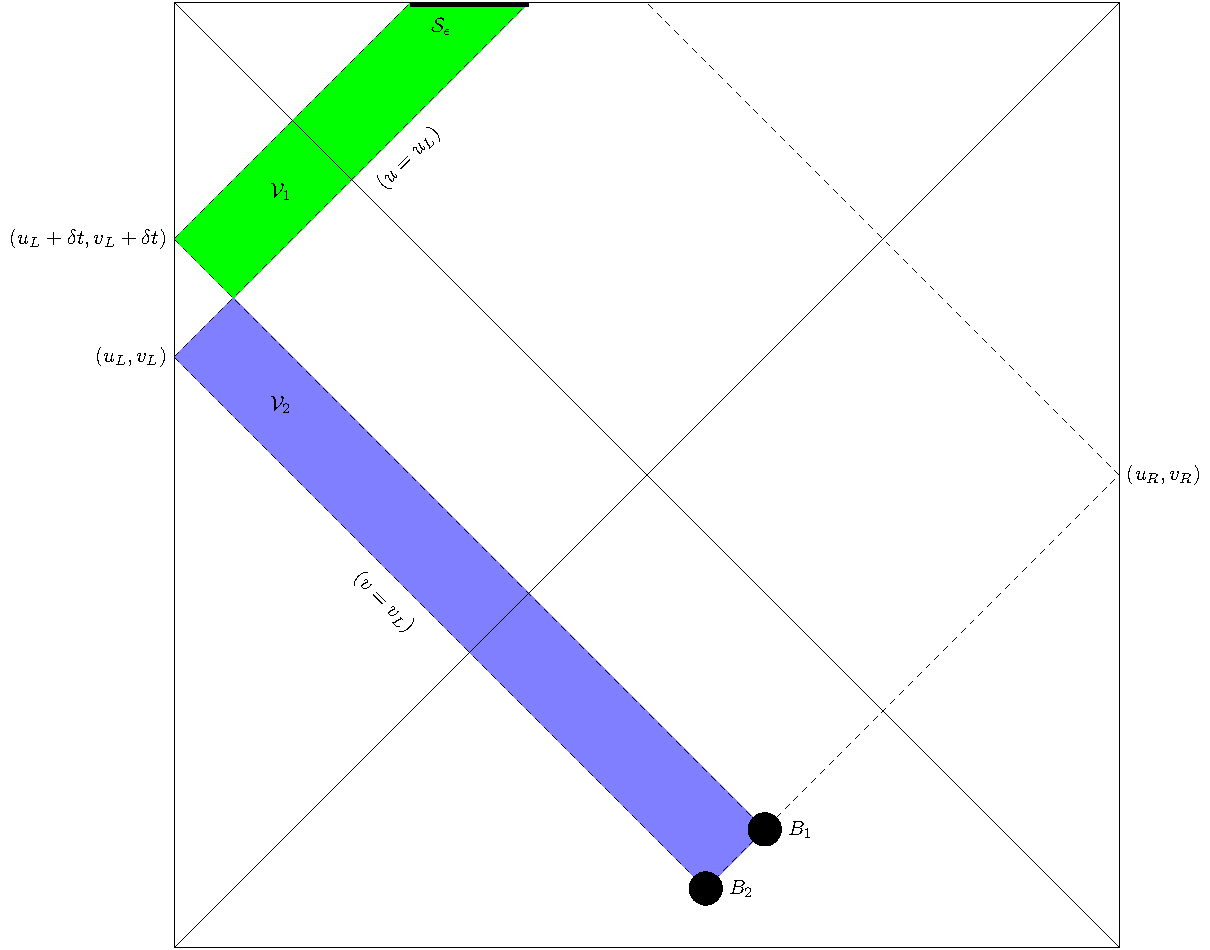
\includegraphics[scale=0.35]{2WDW.pdf}    
    
    \end{center}
    \caption{Two WDW patches separated by $\delta t$.  In thi figure, we have suppressed the cutoff}
    \label{fig:2WDW}
\end{figure}

\end{minipage}

\end{frame}

\section{Holographic Complexity and Non-Commutative Field Theory}

\subsection{Introduction}

\begin{frame}
\frametitle{Introduction}

It would be nice to have a first principles derivation of the holographic dual of circuit complexity. Unfortunately, this has not yet been done and is probably hard to do. In the absence of such a derivation, we would like to have some novel contexts where we can 'test' the holographic complexity by comparing to expected behaviour.

\begin{itemize}

\item One possibility we will discuss here is non-commutative field theory, i.e. field theory living on a non-commutative manifold

\item In particular, we will be interested in Non-commutative ($\mathcal{N}=4$) super Yang-Mills (NCSYM).

\item A gravity solution dual to NCSYM was derived in by a number of authors by Hashimoto and Itzhaki (1999) and was later discussed by Maldacena and Russo (1999).

%\item And this solution has been well studied in other contexts (see e.g. Cai et al. \cite{Cai:1999aw}, Edlati et al. \cite{Edalati:2012jj}, Fischler et al. \cite{Fischler:2013gsa}, Karczmarek et al. \cite{Karczmarek:2013xxa}).

\begin{itemize}
		
	\item Themodynamics (Cai \& Ohta (2000), Fischler et al. (2000))
	\item Fast Scambling (Edalati et al. (2012))
	\item Entanglement entropy (Fischler et al. (2013), Karczmarek et al. (2013))
	
\end{itemize}

\item Also, generalizations of this system to other numbers of dimensions have also been considered in, e.g., Alishahiha et al. (1999) and Berman et al. (1999).

\end{itemize}

\end{frame}

\subsection{NCSYM and its Gravity Dual}

\begin{frame}
\frametitle{Non-Commutative Geometry}

What is a non-commutative manifold?

\begin{itemize}

\item A manifold in which the coordinates are taken to be non-commuting, i.e. given coordinates $x_i$ and $x_j$, we introduce a non-trivial commutator $[x_i,x_j]$ between them.

\item Ordinary quantum mechanics is a theory on a non-commutative manifold, where the manifold $\mathcal{M}$ is the symplectic manifold of a Hamiltonian system and $[x_i,x_j] = i \hbar \text{ } \omega^{ij} x_i x_j$, where $\omega$ is the symplectic form on $\mathcal{M}$.

\item One may do quantum mechanics on a non-commutative spatial manifold by introducing a non-zero commutator between distinct directions, e.g. in 2 dimensions we can have $[x,y] = i a^2$. In this case $a$ is called the \textit{Moyal scale}

\item This new commutator implies a new uncertainty relation $\Delta x \Delta y \geq i a^2$, and so particles cannot be localized at spatial scales larger smaller than $a$. This is one way of seeing that non-commutative theories are non-local.

\item One may define fields on a non-commutative manifold by replacing ordinary products of fields $\phi(x) \psi(y)$ by the so-called Moyal product: $(\phi * \psi)(x) = \exp(i a^2 \nabla_x \nabla_{x'}) \phi(x) \psi(x') \bigg|_{x'=x}$

\item The theory of charges in a conducting sheet with a normal magnetic field (A quantum Hall system) becomes non-commutative when restricted to the lowest Landau level.

\end{itemize}

\end{frame}

\begin{frame}
\frametitle{The gravity dual to NCSYM}

The gravity dual to NCSYM is obtained in a manner similar to that of standard $\mathcal{N} = 4$ SYM.

\begin{itemize}

\item Consider a stack of D3-branes

\item We turn on a 2-form B parallel to the two spatial dimensions of the branes

\item This can be achieved by applying a combination of T-dualities and Gauge transformations

\item The B-field has the effect of introducing non-commutativity in the worldbrane theory

\item The near horizon geometry in the usual limit gives the gravity dual, which is a IIB SUGRA solution.

\end{itemize}

The resulting solution, at finite teperature, is given in Einstein frame as follows:

\begin{equation}
ds^2 = \alpha' \bigg[ \left(\frac{r}{L}\right)^2
\left(- f(r) dt^2 + dx_1^2  + h(r) (dx_2^2 + dx_3^2)\right)
+\left(\frac{L}{r}\right)^2 \left(
\frac{dr^2}{f(r)} + r^2 d\Omega_5^2\right)\bigg],
\end{equation}
%
\begin{equation}
e^{2\Phi} = \hat{g}_s^2 h(r) ,\quad B_{23} = B_{\infty}(1-h(r)) ,\quad C_{01} = -\frac{\alpha^{\prime} a^2 r^4}{\hat{g}_s R^2} ,\quad F_{0123r} = \frac{4\alpha^{\prime 2} r^3}{\hat{g}_s R^4} h(r)
\end{equation}
%
\begin{equation}
f(r) = 1 - \left(\frac{r_+}{r}\right)^4 ,\quad h(r) = \frac{1}{1 + a^4 r^4} ,\quad B_{\infty} = -\frac{\alpha'}{a^2 L^2}. 
\end{equation}

Here $L$ is the AdS length scale, $r_+$ is the bulk coordinate of the horizon, $\hat{g}_s$ is the  and closed string coupling, and $a$ is the Moyal scale (i.e. $[x_2,x_3]= i a^2$ on the boundary).

\end{frame}

\begin{frame}
\frametitle{The gravity dual to NCSYM}

A few additional notes about the gravity dual:

\begin{itemize}

\item The bulk coordinate $r$ has units of inverse length.

\item Though the boundary field theory lives on a non-commutative manifold, the bulk geometry is commutative.

\item The metric degenerates at the boundary. This should be fine, however, provided we always work with a finite cutoff.

\item The dimension of the Hilbert space in the dual theory was found to be independent of the Moyal scale by Maldacena and Russo (1999).

\end{itemize}

We will now consider an intuition based heuristic argument that we should expect the complexity at a given (late) time should be higher in NCSYM than in it's commutative counterpart.

\end{frame}

\subsection{Effect of Non-Locality on Complexity}

\begin{frame}
\frametitle{Non-Commutativity and Complexity: A heuristic argument}

\begin{minipage}[t]{0.5\linewidth}

\begin{itemize}

\item Consider the unitary operator $U$ which translates our state in time by a small time $\delta t$. 

\end{itemize}

\end{minipage}\hfill
%
\begin{minipage}[t]{0.48\linewidth}

\begin{figure}
    \begin{center}
    
        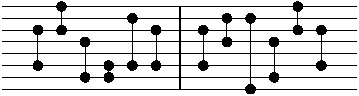
\includegraphics[scale=1]{animation/animation_1}    
        
        \vspace{2mm}
        
        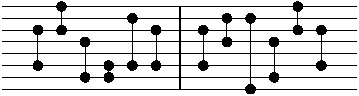
\includegraphics[scale=1]{animation/animation_1}    
    
    \end{center}
    \caption{A small piece of a circuit implementing time translations on a local (top) and non-local (bottom) theory. This cartoon is inspired by another which appears in certain talks by Adam Brown.}
\end{figure}

\end{minipage}

\end{frame}


\begin{frame}
\frametitle{Non-Commutativity and Complexity: A heuristic argument}

\begin{minipage}[t]{0.5\linewidth}

\begin{itemize}

\item Consider the unitary operator $U$ which translates our state in time by a small time $\delta t$. 

\item Consider further an optimal circuit $Q$ implementing $U$.

\end{itemize}

\end{minipage}\hfill
%
\begin{minipage}[t]{0.48\linewidth}

\begin{figure}
    \begin{center}
    
        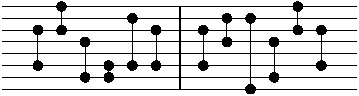
\includegraphics[scale=1]{animation/animation_1}    
        
        \vspace{2mm}
        
        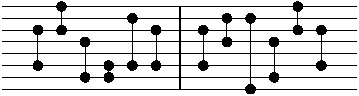
\includegraphics[scale=1]{animation/animation_1}    
    
    \end{center}
    \caption{A small piece of a circuit implementing time translations on a local (top) and non-local (bottom) theory. This cartoon is inspired by another which appears in certain talks by Adam Brown.}
\end{figure}

\end{minipage}

\end{frame}


\begin{frame}
\frametitle{Non-Commutativity and Complexity: A heuristic argument}

\begin{minipage}[t]{0.5\linewidth}

\begin{itemize}

\item Consider the unitary operator $U$ which translates our state in time by a small time $\delta t$. 

\item Consider further an optimal circuit $Q$ implementing $U$.

\item At late time $t$, the circuit $Q^N$ approximates $U^N$, where $N= t/\delta t$.

\end{itemize}

\end{minipage}\hfill
%
\begin{minipage}[t]{0.48\linewidth}

\begin{figure}
    \begin{center}
    
        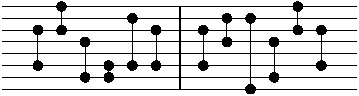
\includegraphics[scale=1]{animation/animation_1}    
        
        \vspace{2mm}
        
        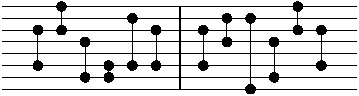
\includegraphics[scale=1]{animation/animation_1}    
    
    \end{center}
    \caption{A small piece of a circuit implementing time translations on a local (top) and non-local (bottom) theory. This cartoon is inspired by another which appears in certain talks by Adam Brown.}
\end{figure}

\end{minipage}

\end{frame}


\begin{frame}
\frametitle{Non-Commutativity and Complexity: A heuristic argument}

\begin{minipage}[t]{0.5\linewidth}

\begin{itemize}

\item Consider the unitary operator $U$ which translates our state in time by a small time $\delta t$. 

\item Consider further an optimal circuit $Q$ implementing $U$.

\item At late time $t$, the circuit $Q^N$ approximates $U^N$, where $N= t/\delta t$.

\item This circuit is generally non-optimal however, as there will be gates which cancel between the beginning and end of successive copies of $Q$.

\end{itemize}

\end{minipage}\hfill
%
\begin{minipage}[t]{0.48\linewidth}

\begin{figure}
    \begin{center}
    
        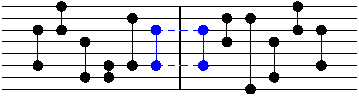
\includegraphics[scale=1]{animation/animation_2}    
        
        \vspace{2mm}
        
        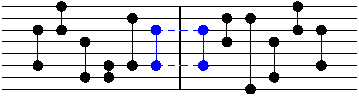
\includegraphics[scale=1]{animation/animation_2}    
    
    \end{center}
    \caption{A small piece of a circuit implementing time translations on a local (top) and non-local (bottom) theory. This cartoon is inspired by another which appears in certain talks by Adam Brown.}
\end{figure}

\end{minipage}

\end{frame}


\begin{frame}
\frametitle{Non-Commutativity and Complexity: A heuristic argument}

\begin{minipage}[t]{0.5\linewidth}

\begin{itemize}

\item Consider the unitary operator $U$ which translates our state in time by a small time $\delta t$. 

\item Consider further an optimal circuit $Q$ implementing $U$.

\item At late time $t$, the circuit $Q^N$ approximates $U^N$, where $N= t/\delta t$.

\item This circuit is generally non-optimal however, as there will be gates which cancel between the beginning and end of successive copies of $Q$.

\item These cancelations lead to a circuit for the same operator of lower complexity

\end{itemize}

\end{minipage}\hfill
%
\begin{minipage}[t]{0.48\linewidth}

\begin{figure}
    \begin{center}
    
        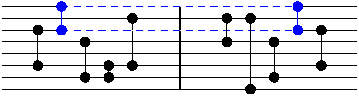
\includegraphics[scale=1]{animation/animation_3}    
        
        \vspace{2mm}
        
        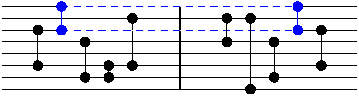
\includegraphics[scale=1]{animation/animation_3}    
    
    \end{center}
    \caption{A small piece of a circuit implementing time translations on a local (top) and non-local (bottom) theory. This cartoon is inspired by another which appears in certain talks by Adam Brown.}
\end{figure}

\end{minipage}

\end{frame}


\begin{frame}
\frametitle{Non-Commutativity and Complexity: A heuristic argument}

\begin{minipage}[t]{0.5\linewidth}

\begin{itemize}

\item Consider the unitary operator $U$ which translates our state in time by a small time $\delta t$. 

\item Consider further an optimal circuit $Q$ implementing $U$.

\item At late time $t$, the circuit $Q^N$ approximates $U^N$, where $N= t/\delta t$.

\item This circuit is generally non-optimal however, as there will be gates which cancel between the beginning and end of successive copies of $Q$.

\item These cancelations lead to a circuit for the same operator of lower complexity

\item In a non-local theory (such as a non-commutative theory), fewer operators commute past one another, and so there will be more obstruction to such cancelations, leading to a higher final complexity.

\end{itemize}

\end{minipage}\hfill
%
\begin{minipage}[t]{0.48\linewidth}

\begin{figure}
    \begin{center}
    
        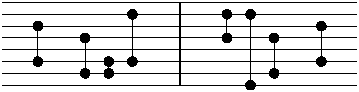
\includegraphics[scale=1]{animation/animation_4}    
        
        \vspace{2mm}
        
        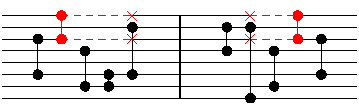
\includegraphics[scale=1]{animation/animation_5}    
    
    \end{center}
    \caption{A small piece of a circuit implementing time translations on a local (top) and non-local (bottom) theory. This cartoon is inspired by another which appears in certain talks by Adam Brown.}
\end{figure}

\end{minipage}

\end{frame}

\subsection{Results and Conclusions}

\begin{frame}
\frametitle{Results}

Now that we have this na\"ive expectation, we will compare with the complexity in NCSYM according to CA. We will find it convenient to define the parameters $b = a r_+ = \pi a T$,  $\rho = \frac{r_B}{r_+}$, and  $\gamma = \frac{c \bar{c} \sqrt{\bar{g}_s} L^2}{\alpha' \pi^2 T^2}$.
\begin{itemize}

\item $T=\pi r_+$ is the temperature

\item $c$ and $\bar{c}$ are the normalizations of the null generators

\end{itemize}

With these conventions, the complexification rate after the critical time is given by

\begin{equation}
\dot{C} = \frac{\Omega_5 V_3 r_+^4}{(2\pi)^7 \hat{g}_s^2}
\bigg(\frac{-2\log(1+b^4 \rho^4)}{b^4}+4\rho^4+6+3(1-\rho^4)\log\big|\frac{\gamma \rho^2}{(1+b^4 \rho^4)^{1/4}(1-\rho^4)}\big|\bigg).
\end{equation}

Here $V_3$ is the volume of a spatial slice of the boundary theory (which is infinite) and $\Omega_3$ is the volume of a unit 5-sphere. In what follows, we will normalize the rates by the $b=0$ result. 

\end{frame}

\begin{frame}
\frametitle{D3-brane results: Finite time behavior}

In the commutative limit, we see similar behavior to that reported by Carmi et al. (2017).

\begin{minipage}[t]{0.48\linewidth}

\begin{itemize}

\item Logarithmic divergence at the critical time.

\item Reaches true global maximum in order one time (in thermal units).

\item approaches asymptotic value from above.

\end{itemize}

This behavior persists for all values of the Moyal scale  but as the Moyal scale becomes very large, the true maximum shrinks and the asymptotic value increases, so that the gap between them decreases

\end{minipage}
%
\begin{minipage}[t]{0.48\linewidth}

\begin{figure}
    \begin{center}
        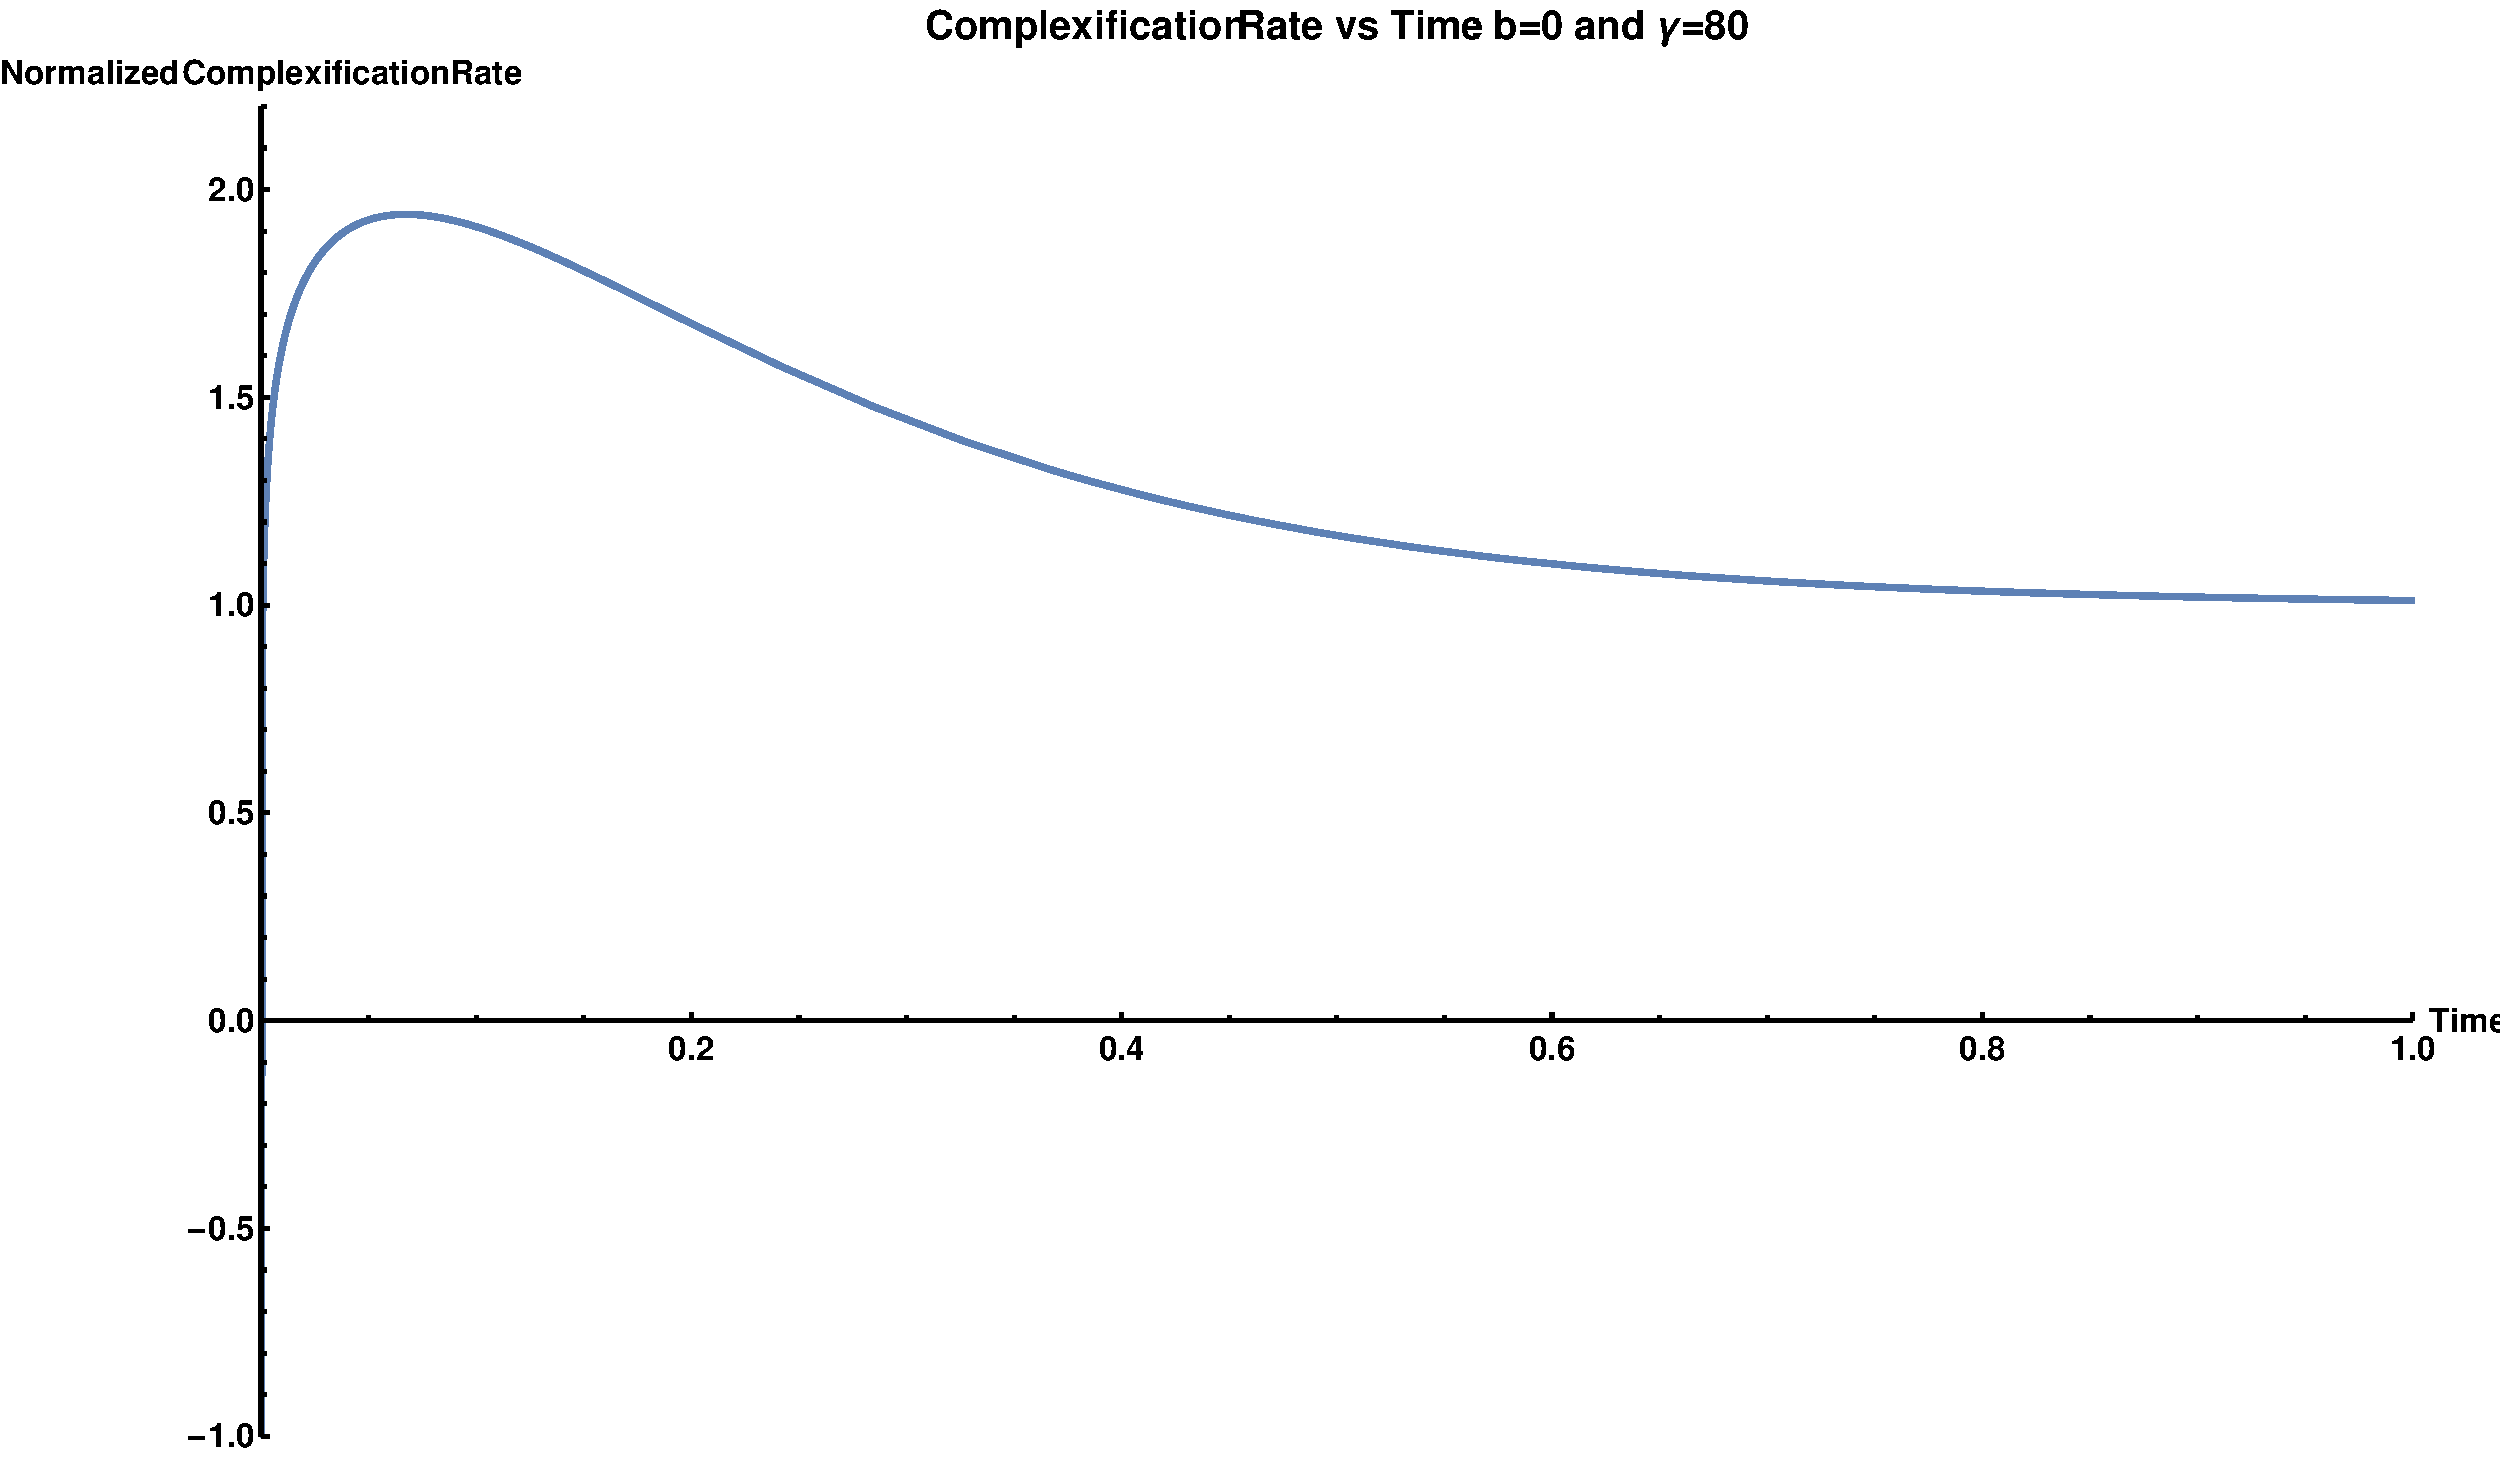
\includegraphics[scale=0.15]{FiniteTime1}
    \end{center}
\end{figure}

\end{minipage}
\vspace{5mm}

This behavior calls into question the normalization to complexity = action as set by Brown et al. (2015), though the logic that to that normalization would seem already to be contradicted by Cottrell and Montero (2017).

\end{frame}

\begin{frame}
\frametitle{Finite time behavior}

Here we see how the finite time behavior changes as we vary the parameters.

\begin{minipage}[t]{0.47\linewidth}

\begin{figure}
    \begin{center}
        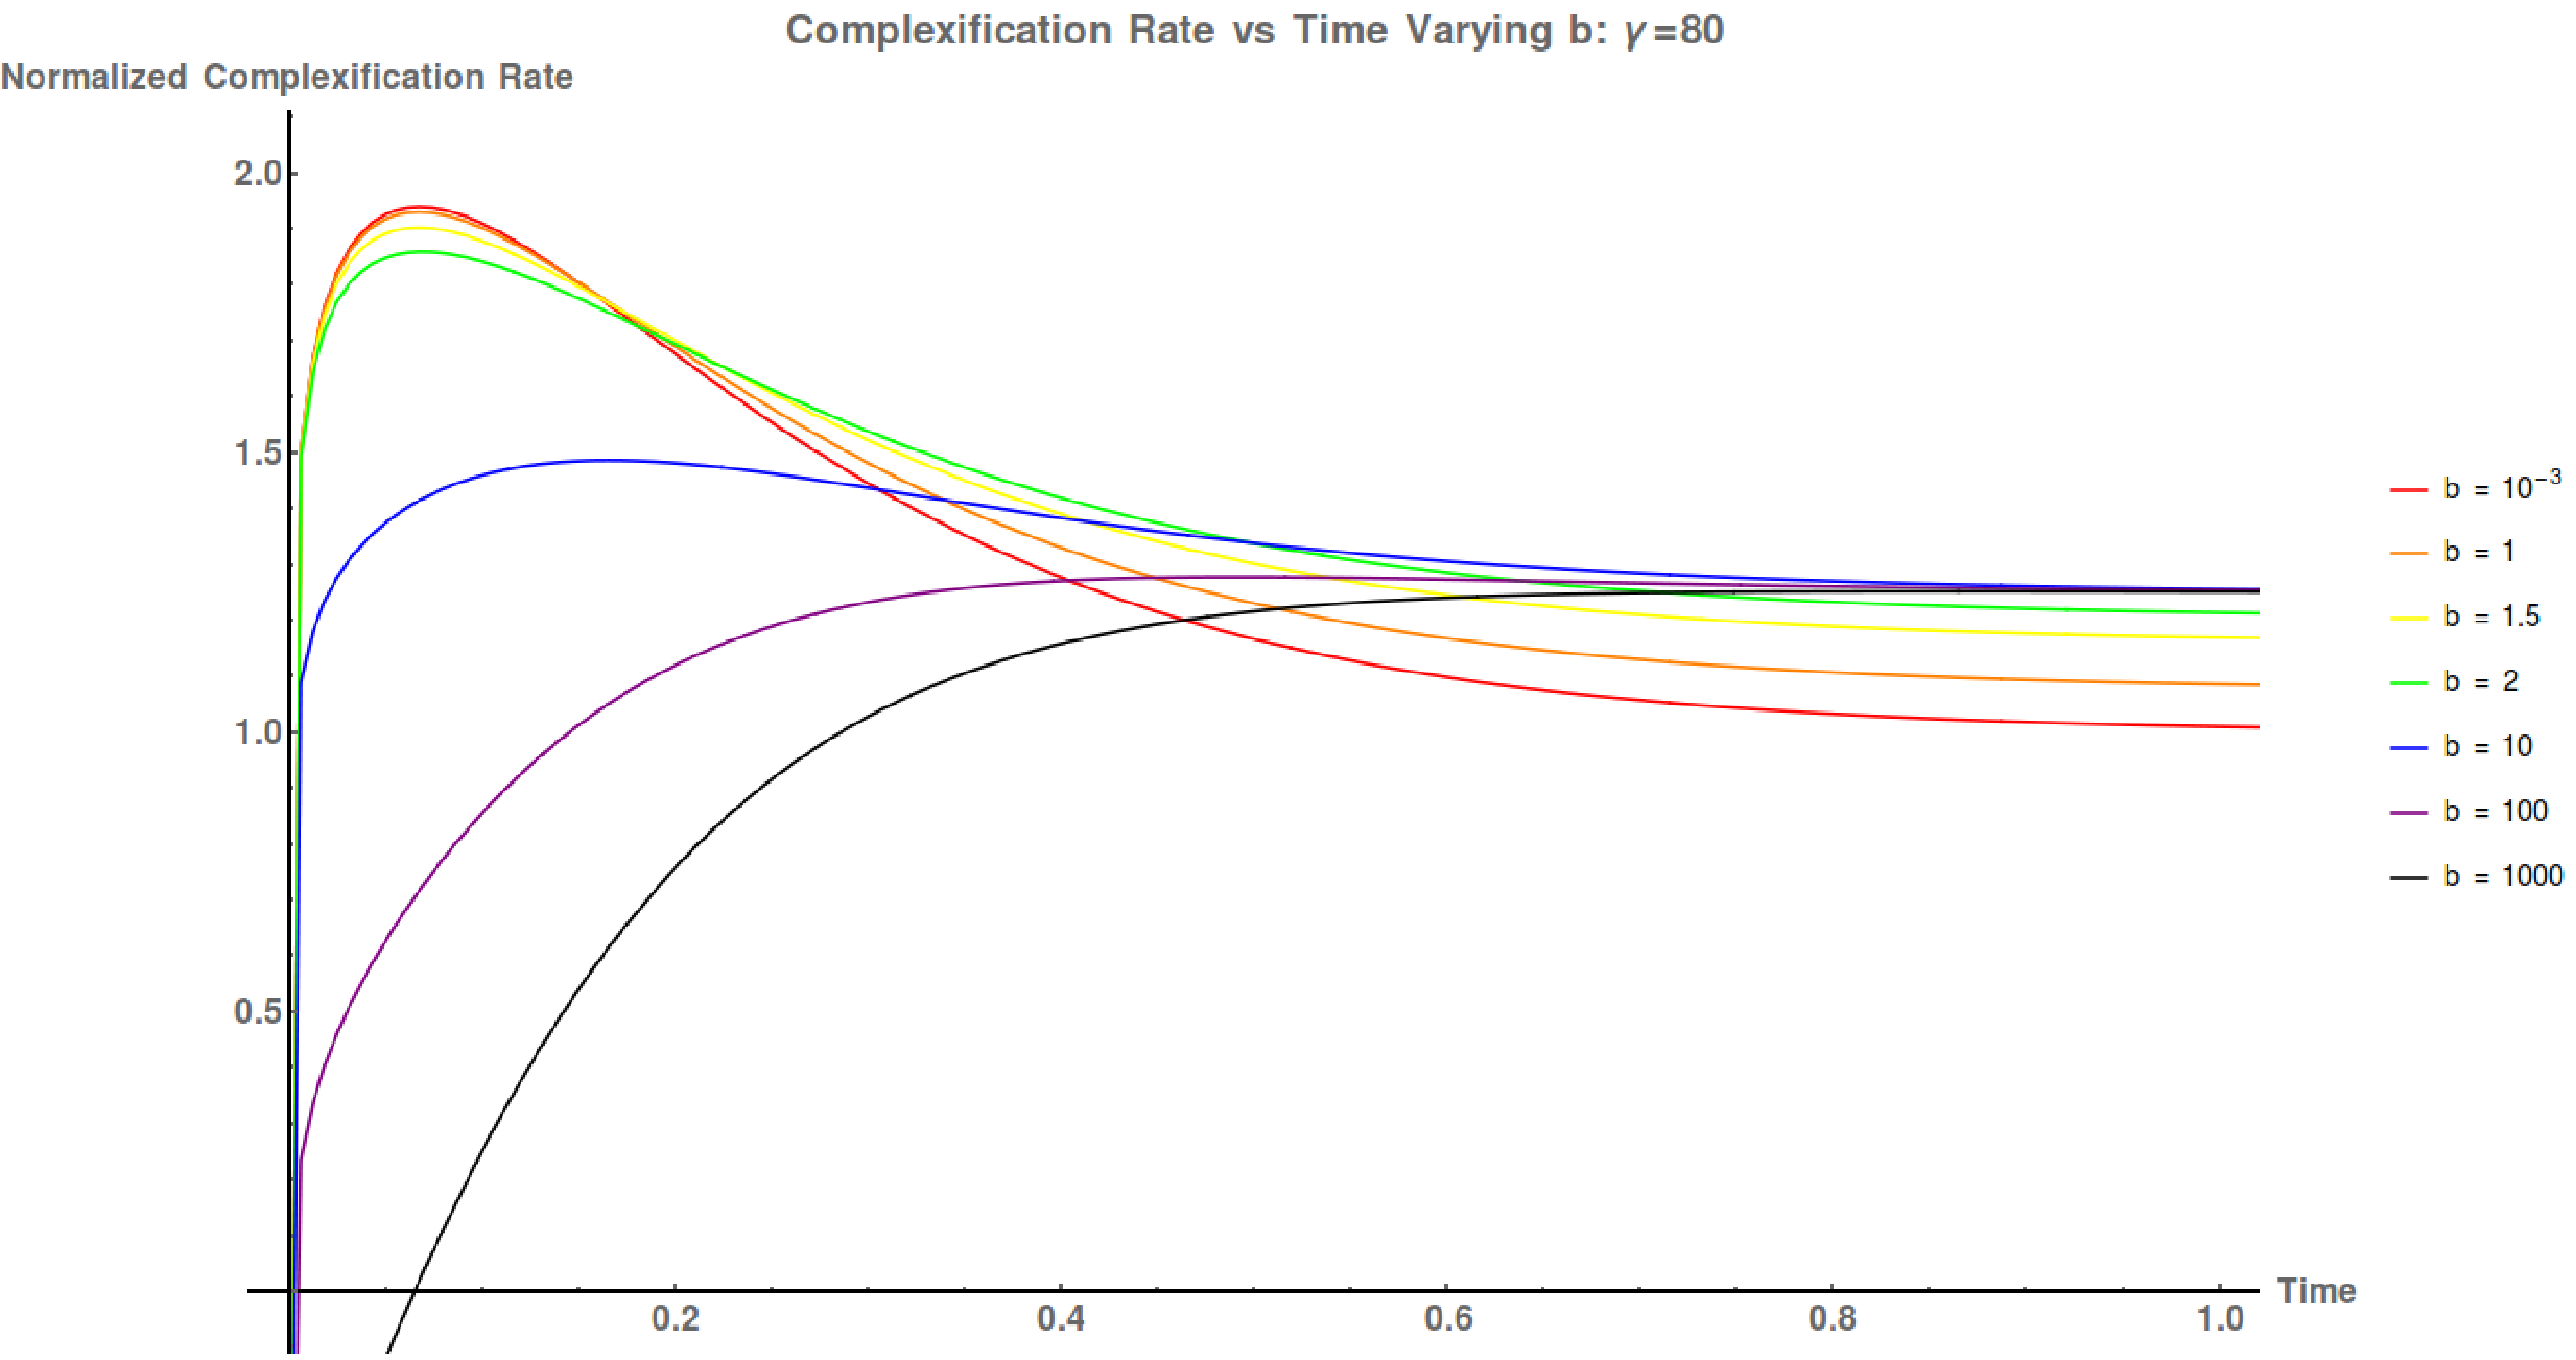
\includegraphics[scale=0.15]{vary_b_fix_gamma}
    \end{center}
\end{figure}

\end{minipage}\hfill
%
\begin{minipage}[t]{0.47\linewidth}

\begin{figure}
    \begin{center}
        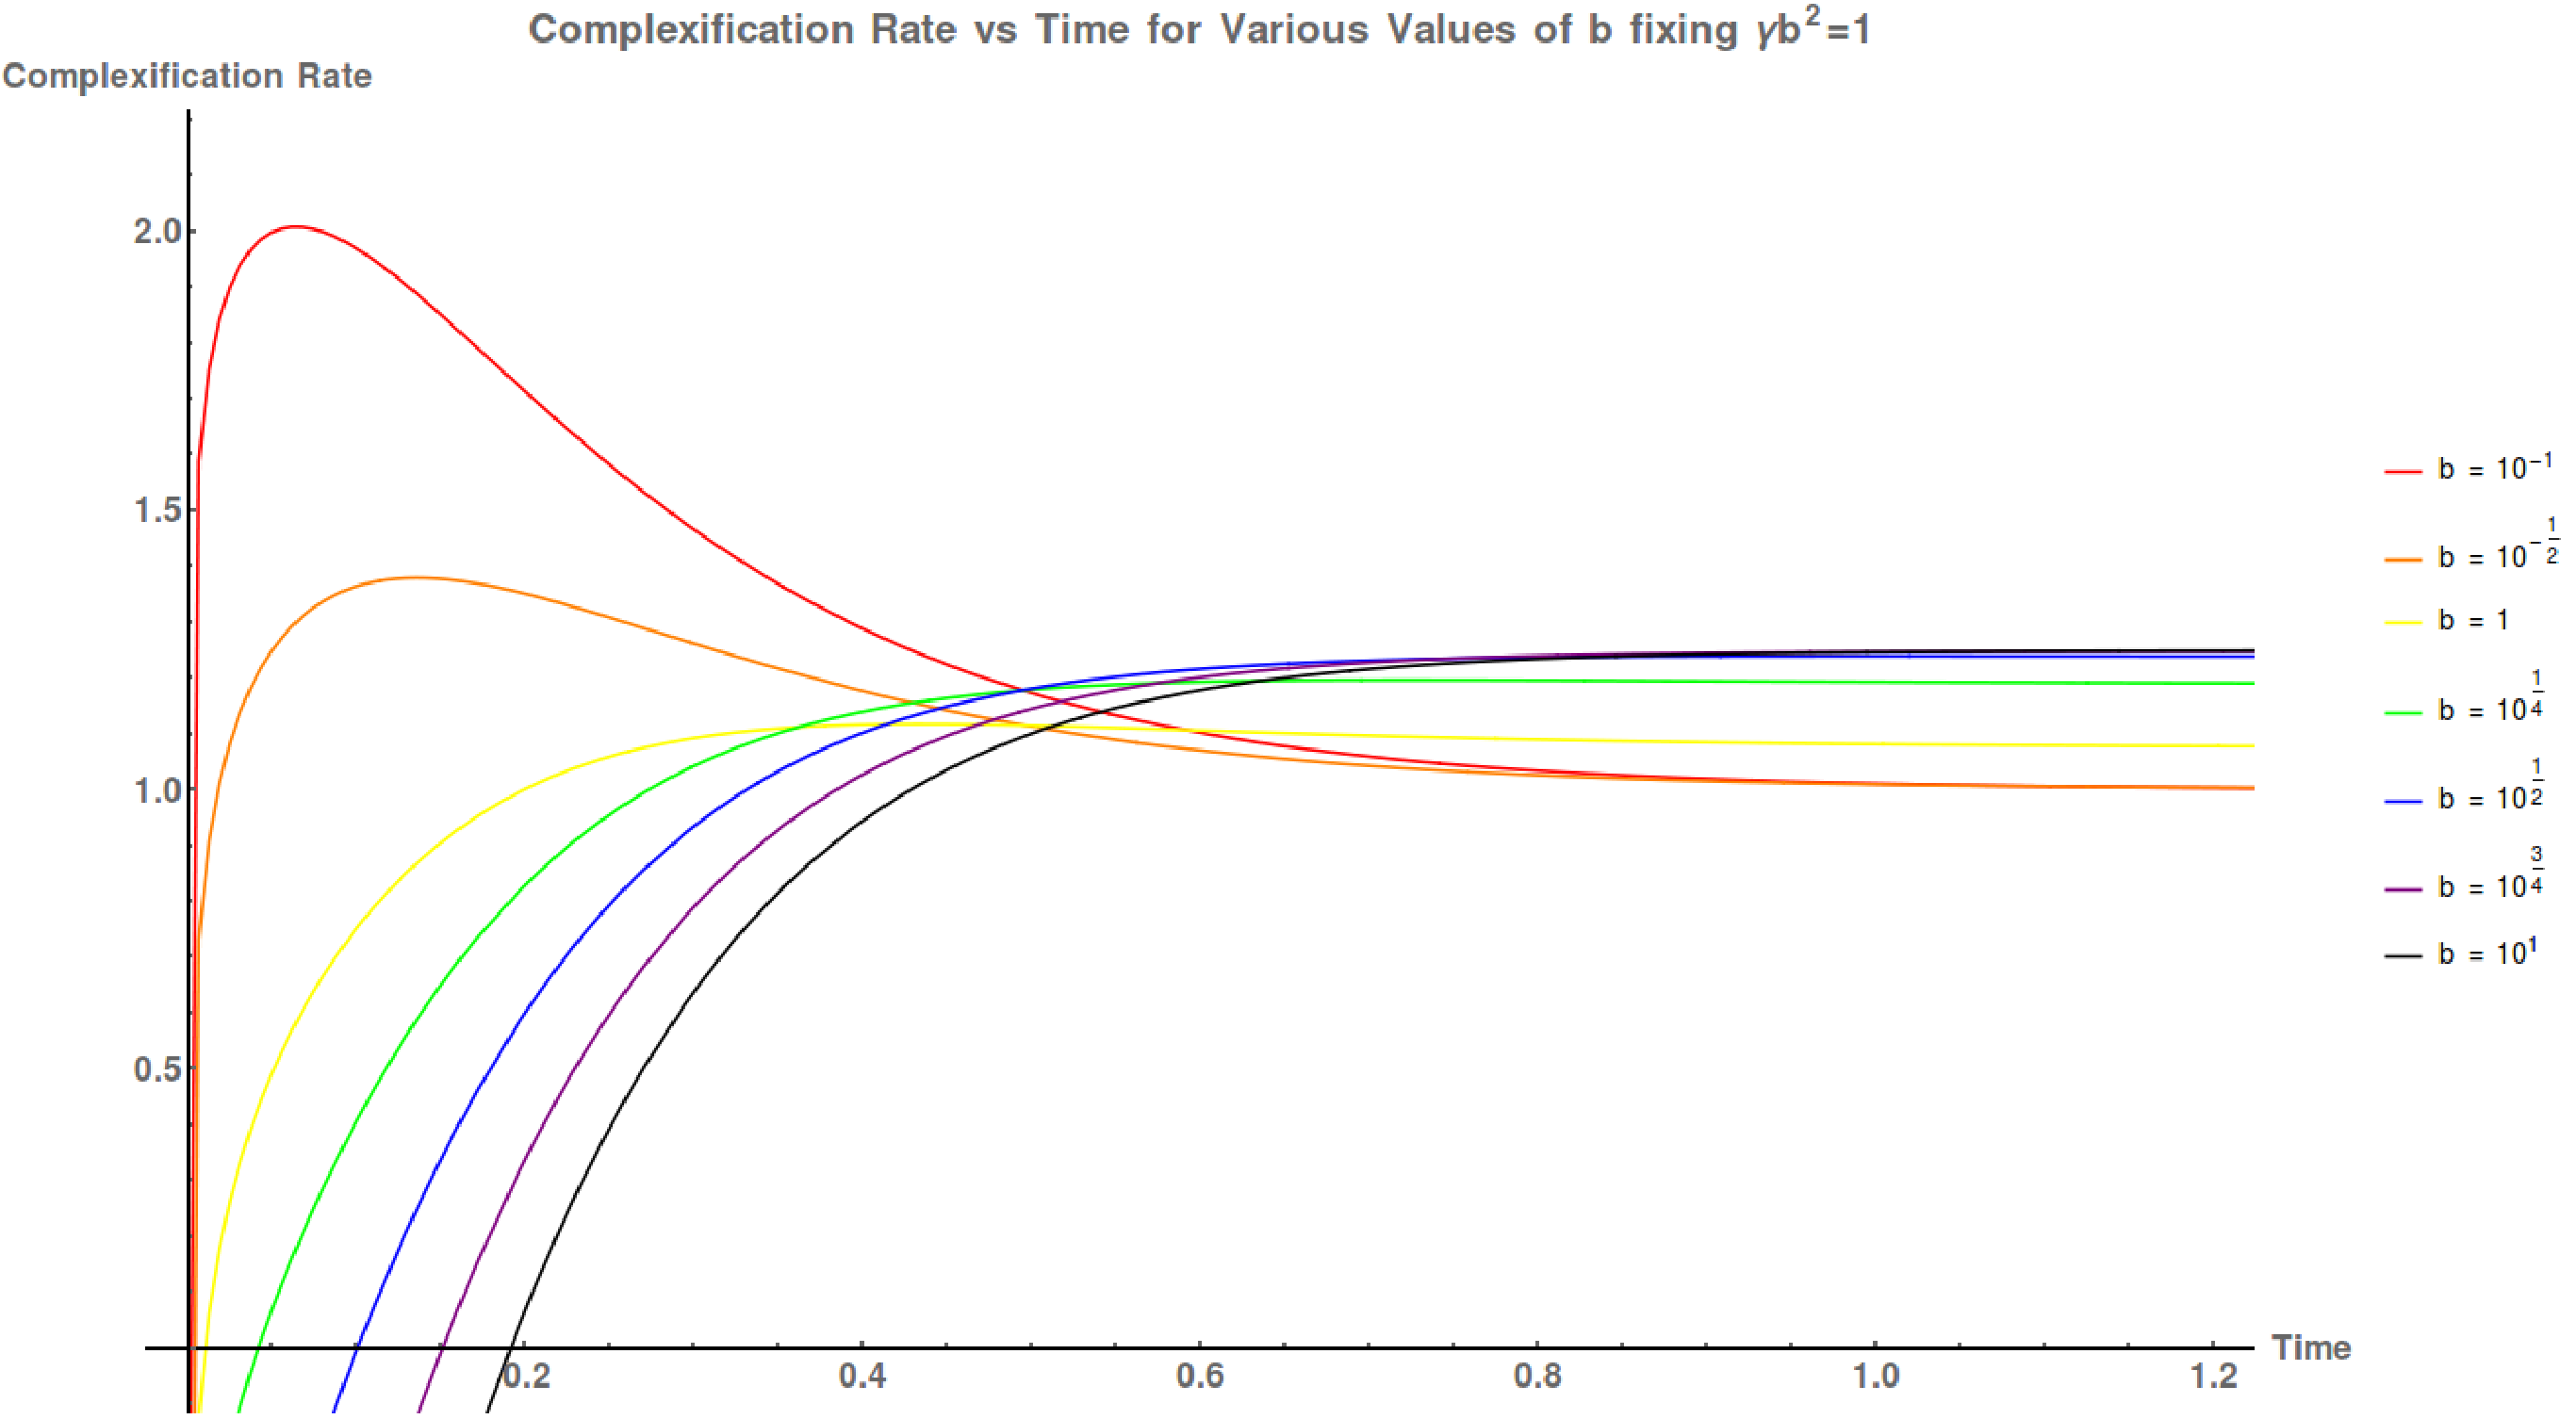
\includegraphics[scale=0.15]{vary_temp}
    \end{center}
\end{figure}

\end{minipage} 

\end{frame}

\begin{frame}
\frametitle{D3-brane results: Late time limit}

We take the late time limit by sending $r_b$ to $r_+$ (i.e. we send $\rho$ to 1). In this limit, the normalized complexification rate becomes

\begin{equation}
\dot{C}_{\text{normalized}} \large|_{t\rightarrow \infty} = \frac{5}{4}-\frac{\log(1+b^4)}{4 b^4}.
\end{equation}

Recalling that $b = \pi a T$, we see that at a fixed temperature, as we send the Moyal scale to infinity, we get $5/4$, which given the normalization scheme tells us that we get exactly a 25\% enhancement in of the complexification rate in the large Moyal scale regime.

\begin{figure}[htbp]
    \begin{center}
        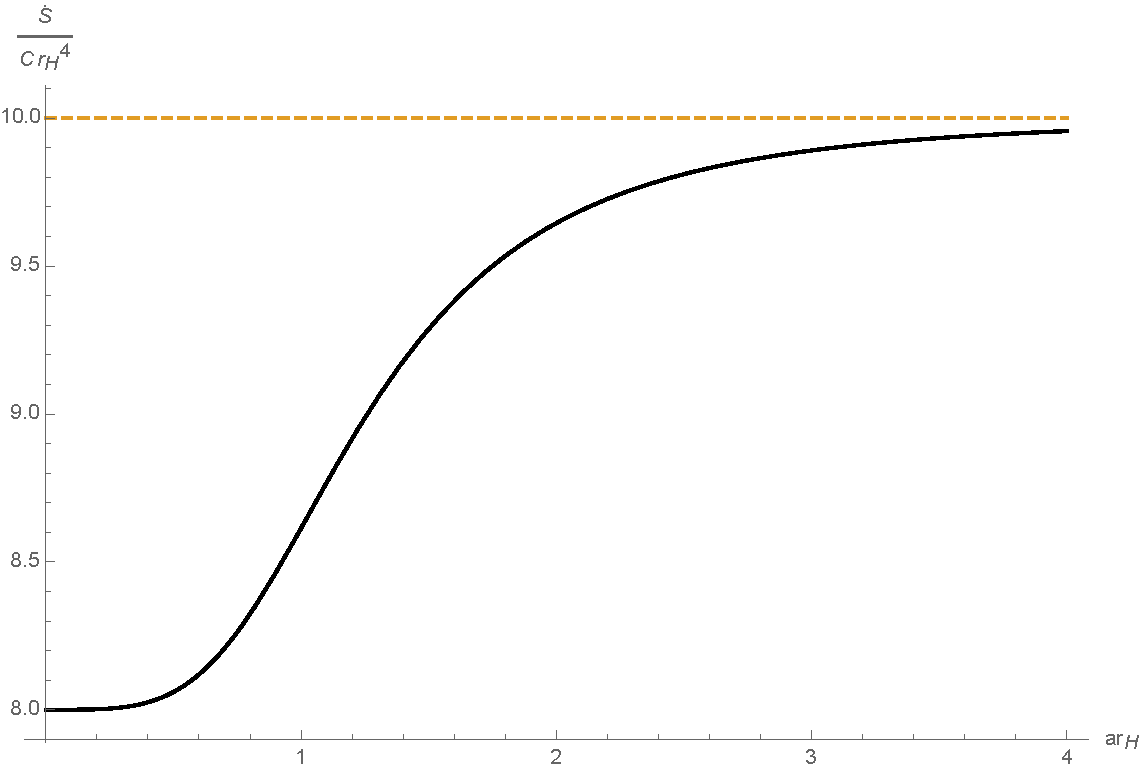
\includegraphics[scale=0.3]{LateTime}
    \end{center}
    \caption{Late time action growth rate normalized by $C=\frac{\alpha^4 \Omega_5 V_3}{\hat{g}_s^2}$ and extra $r_H$ dependence, versus $a r_+$, which is the Moyal scale measured in units of thermal length.} 
    \label{fig:LateTime}
\end{figure}

\end{frame}

\begin{frame}
\frametitle{Results for other values of $p$}

As discussed before, the geometry we have considered so far can be generalized by starting with stacks of $Dp-branes$ with for other values of $p$. For $p\neq 3$, the resulting geometry is not asymptotically AdS, even in the commutative limit. We considered $2\leq p \leq 5$. For $p\geq 4$ there is the possibility of introducing non-commutativity between multiple pairs of coordinates. The table below summarizes our results for the late time rate of change of the complexity density, with a common normalization for all results. Here $m$ indicates the number of pairs of non-commuting coordinates on the boundary.   

\begin{table}
    \centering
    \begin{tabular}{l | c  c  c }
        $p$ & $m=0$ & $m=1$ & $m=2$ \\
        \hline
        2 & 12 & 12 & - \\
        3 & 8 & 10 & - \\
        4 & 5 & 5 & 8 \\
        5 & 4 & 5 & 6 \\
    \end{tabular}
\end{table}

\end{frame}

\begin{frame}
\frametitle{Conclusions}

\begin{itemize}

\item For $p=3,5$ we do see an increase at late time, as expected.

\item Though we did not see an increase for $p=2$ or for $p=4$ with a single non-trivial commutator, at least we did not see a decrease either.

\item Overall, the results are consistent with the heuristic argument above.

\item This result is in tension with the idea that commutative black holes are the fastest possible computers

\item In future work, we plan to repeat our calculations for complexity = volume.

\end{itemize}

\end{frame}

%\section{Complexity = Action and Extended BH Thermodynamics}

%\subsection{Extended BH Thermodynamics}

%\begin{frame}
%\frametitle{(Extended) BH Thermodynamics}

%\begin{itemize}

%\item BH thermodynamics

%\end{itemize}

%\end{frame}

%\subsection{The Extended First Law}

%\subsection{Complexity and Extended Thermodynamics}

%\subsection{Complexity = Spacetime Volume?}

\section{Further/Future work}

\begin{frame}
\frametitle{Further Work}

A few other things we are thinking about in Holographic Complexity:

\begin{itemize}

\item Geometric properties of maximal volumes:

\begin{itemize}

	\item A 'second law' for complexity behind a future horizon.
	
	\item Positivity of mixed time  derivative $\rightarrow$ monotonicity of complexification rate.
	
	\item super-additivity

\end{itemize}

\item Mixed state complexity from field theory.

\item Complexity and holographic complexity in other non-local field theories

\end{itemize}

\end{frame}

%\begin{frame}
%\frametitle{References}
%{\tiny
%\bibliographystyle{JHEP} %JHEP.bst
%\footnotesize\bibliography{Notes} %NCG.bib
%}
%\end{frame}

\end{document}